\chapter{The Fourier Transform, Sampling and the Periodogram}\label{ch:fourier-transform}

\begin{chapterintro}
In Chapter~\ref{ch:fourier-series} you learned to break a \emph{periodic} function into sines and cosines. Most signals you will ever analyze are not periodic, and you only ever see them over a finite stretch. A single drum hit, the ring-down of a tuning fork and the fluctuating part of the Riemann zeros are all like this. The zeros are a particularly awkward case. We know a finite list of heights $t_1,t_2,\dots,t_{10000}$; they are spaced irregularly; and their fluctuation is a sum of oscillations whose frequencies, $\log 2$, $\log 3$, $\log 4$, \dots, have no common period, so the pattern never repeats exactly.

This chapter builds the tools for asking ``which frequencies are present?'' about such data. We let the period of a Fourier series grow without limit to obtain the \emph{Fourier transform}. We then work out what a \emph{finite} observation window does to a spectrum: every sharp frequency is smeared into a ``sinc'' shape of width about $2\pi/T$, where $T$ is the window length, and energy leaks into neighboring frequencies. We treat sampling, both uniform (where aliasing appears) and irregular (as for the zeros), the discrete Fourier transform and its fast algorithm, the periodogram and how to find its peaks, the autocorrelation of a sequence and its link to the power spectrum (the Wiener--Khinchin theorem), and finally \emph{phase randomization}, which manufactures fake data with exactly the same power spectrum as the real data.

Where this shows up in the paper: the fitted sinusoidal controls C1 and C2 of Sec.~II~D (a uniform frequency grid; a periodogram peak search on $0.05<\omega<8$), the phrase ``within half the Fourier resolution'' of Sec.~IV, the shuffled and phase-randomized surrogate targets of Sec.~III, the remark in Sec.~IV that ``the Fourier transform of the zeros is concentrated at logarithms of prime powers'', and steps 18, 20 and 23 of Appendix~A.
\end{chapterintro}

\begin{prerequisites}

\item Complex numbers, the complex exponential $e^{i\theta}=\cos\theta+i\sin\theta$, modulus, argument, conjugate and the triangle inequality $\abs{z_1+z_2}\le\abs{z_1}+\abs{z_2}$ (Chapter~\ref{ch:complex}).
\item Partial sums and the finite geometric series $\sum_{j=0}^{N-1}r^j=(1-r^N)/(1-r)$ for $r\neq1$ (Chapter~\ref{ch:series}).
\item Big-$\mathcal O$ notation and comparing sums with integrals (Chapter~\ref{ch:asymptotics}).
\item Fourier series in real and complex form, orthogonality of $e^{ik\omega t}$ over a period, Parseval's relation, and almost periodic sums such as $\sin(t\log2)+\sin(t\log3)$ (Chapter~\ref{ch:fourier-series}).
\item First-year physics: angular frequency, period, superposition of waves, beats; single-variable calculus including integration by parts and substitution.

\end{prerequisites}

%======================================================================
\section{From Fourier series to the Fourier transform}\label{sec:fourier-transform-def}

A plucked guitar string vibrates periodically, and Chapter~\ref{ch:fourier-series} showed that a periodic motion is a sum of harmonics at multiples of one fundamental frequency. Now think of a single clap of the hands. It happens once. It has no period, yet your ear still hears it as ``high'' or ``low''; it has a frequency content. We want a definition of frequency content that does not need a period.

The idea is simple: treat a non-periodic function as a periodic one whose period is so long that the next repetition never arrives.

\subsection{Letting the period grow}

Recall from Chapter~\ref{ch:fourier-series} the complex Fourier series. If $f(t)$ has period $T$, then
\begin{equation}
f(t)=\sum_{k=-\infty}^{\infty}c_k\,e^{i\omega_k t},\qquad \omega_k=\frac{2\pi k}{T},
\label{eq:fourier-transform-series}
\end{equation}
with coefficients
\begin{equation}
c_k=\frac1T\int_{-T/2}^{T/2}f(t)\,e^{-i\omega_k t}\,\dd t .
\label{eq:fourier-transform-coeff}
\end{equation}
Here $t$ is the independent variable (time for a clap; for the zeros, the height $t$ of a zero $\tfrac12+it$, where the line of complex numbers with real part $\tfrac12$ is called the critical line, Chapter~\ref{ch:zeta}), $k$ is an integer labeling the harmonic, and $\omega_k$ is the angular frequency of harmonic $k$, in radians per unit of $t$.

Now let $f$ be defined on the whole real line, not periodic, and small when $\abs t$ is large. Pick a long interval $[-T/2,T/2]$. The series \eqref{eq:fourier-transform-series} with coefficients \eqref{eq:fourier-transform-coeff} only ``sees'' the values of $f$ inside this interval and reproduces $f$ there (it reproduces outside it the periodic repetition of that piece, which we will not use). Define, for \emph{every} real $\omega$, not only the harmonics,
\begin{equation}
F_T(\omega)=\int_{-T/2}^{T/2}f(t)\,e^{-i\omega t}\,\dd t .
\label{eq:fourier-transform-FT}
\end{equation}
Comparing with \eqref{eq:fourier-transform-coeff}, $c_k=F_T(\omega_k)/T$. The harmonics are spaced by
\begin{equation}
\Delta\omega=\omega_{k+1}-\omega_k=\frac{2\pi}{T},\qquad\text{so}\qquad \frac1T=\frac{\Delta\omega}{2\pi}.
\end{equation}
Substituting into \eqref{eq:fourier-transform-series}, for $\abs t<T/2$,
\begin{align}
f(t)&=\sum_{k}\frac{1}{T}F_T(\omega_k)\,e^{i\omega_k t}\notag\\
&=\frac{1}{2\pi}\sum_{k}F_T(\omega_k)\,e^{i\omega_k t}\,\Delta\omega .
\label{eq:fourier-transform-riemann}
\end{align}
The last line is a Riemann sum: values of the function $F_T(\omega)e^{i\omega t}$ at equally spaced points $\omega_k$, each multiplied by the spacing $\Delta\omega$. As $T\to\infty$ the spacing shrinks to zero, the Riemann sum turns into an integral over $\omega$, and $F_T$ turns into the integral over the whole line. This is a heuristic argument (two limits are taken at once and we have not checked that they may be interchanged), but it tells us what to define.

\begin{equation}
\boxed{\;\hat f(\omega)=\int_{-\infty}^{\infty}f(t)\,e^{-i\omega t}\,\dd t\;}
\label{eq:fourier-transform-def}
\end{equation}
is the \textbf{Fourier transform} of $f$, and the limit of \eqref{eq:fourier-transform-riemann} suggests the \textbf{inverse transform}
\begin{equation}
f(t)=\frac{1}{2\pi}\int_{-\infty}^{\infty}\hat f(\omega)\,e^{i\omega t}\,\dd\omega .
\label{eq:fourier-transform-inv}
\end{equation}
The integral over the whole line means $\lim_{A\to\infty,B\to\infty}\int_{-A}^{B}$, an ``improper'' integral. We call $\hat f(\omega)$ the \emph{spectrum} of $f$; its modulus $\abs{\hat f(\omega)}$ is the \emph{amplitude spectrum} and its argument is the \emph{phase spectrum}. If $t$ were time in seconds, $\omega$ would be in rad/s. In this book $t$ is usually a height on the critical line (a pure number), so $\omega$ is in radians per unit of $t$.

\begin{beyond}
\textbf{Taken on trust: the Fourier inversion theorem.} If $\int_{-\infty}^{\infty}\abs{f(t)}\,\dd t$ is finite and $f$ is piecewise smooth, then \eqref{eq:fourier-transform-inv} holds at every point where $f$ is continuous (at a jump it gives the midpoint of the jump). Our argument above is a motivation, not a proof. A proof at the level of a mathematical-methods course is in \cite{rhb}.
\end{beyond}

\subsection{When does the transform exist?}

Because $\abs{e^{-i\omega t}}=1$ for real $\omega t$, the size of the integrand in \eqref{eq:fourier-transform-def} is $\abs{f(t)}$. The integral of a complex-valued function $g=u+iv$ of the real variable $t$ means $\int u\,\dd t+i\int v\,\dd t$. It is the limit of the Riemann sums $\sum_j g(t_j)\Delta t$, because the real and imaginary parts converge separately. By the triangle inequality $\abs{\sum z_j}\le\sum\abs{z_j}$ of Chapter~\ref{ch:complex}, each Riemann sum satisfies $\abs{\sum_j g(t_j)\Delta t}\le\sum_j\abs{g(t_j)}\Delta t$. The left side tends to $\abs{\int g\,\dd t}$, since the modulus is continuous, and the right side tends to $\int\abs g\,\dd t$. An inequality between two sequences survives in the limit, so $\abs{\int g\,\dd t}\le\int\abs g\,\dd t$. Hence
\begin{equation}
\abs{\hat f(\omega)}\le\int_{-\infty}^{\infty}\abs{f(t)}\,\dd t .
\label{eq:fourier-transform-bound}
\end{equation}
So if $f$ is \emph{absolutely integrable} (the right side is finite), $\hat f(\omega)$ exists and is bounded for every $\omega$. A pure sinusoid $\sin(\omega_0 t)$ is \emph{not} absolutely integrable: the area under $\abs{\sin(\omega_0 t)}$ grows without limit. Its transform does not exist as an ordinary integral. That is not a disaster; it is the first hint that, for oscillations that go on forever, we should look through a finite window (Section~\ref{sec:fourier-transform-window}).

\begin{sample}{The transform of a rectangular pulse}
Find $\hat f(\omega)$ for the ``box'' $f(t)=1$ for $\abs t\le T/2$ and $f(t)=0$ otherwise. Evaluate it for $T=4$ at $\omega=1$, and find where it first vanishes.

\textbf{Step 1: Set up.} The integrand vanishes outside $[-T/2,T/2]$, so
\[\hat f(\omega)=\int_{-T/2}^{T/2}e^{-i\omega t}\,\dd t .\]

\textbf{Step 2: Integrate} (for $\omega\neq0$). An antiderivative of $e^{-i\omega t}$ is $e^{-i\omega t}/(-i\omega)$:
\[\hat f(\omega)=\frac{e^{-i\omega T/2}-e^{i\omega T/2}}{-i\omega}.\]

\textbf{Step 3: Simplify.} From $\sin\theta=(e^{i\theta}-e^{-i\theta})/(2i)$ (Chapter~\ref{ch:complex}), the numerator is $-2i\sin(\omega T/2)$. Dividing by $-i\omega$,
\[\hat f(\omega)=\frac{2\sin(\omega T/2)}{\omega}.\]
At $\omega=0$ the integral is directly $\int_{-T/2}^{T/2}1\,\dd t=T$, which is also the limit of the formula since $\sin x\approx x$ for small $x$.

\textbf{Step 4: Numbers.} With $T=4$ and $\omega=1$: $\hat f(1)=2\sin 2=2\times0.909297=1.8186$. The formula vanishes where $\sin(\omega T/2)=0$ with $\omega\ne0$, i.e.\ $\omega T/2=\pm\pi,\pm2\pi,\dots$; the first zero is at $\omega=2\pi/T=\pi/2=1.5708$.

\[\boxed{\hat f(\omega)=\frac{2\sin(\omega T/2)}{\omega},\quad \hat f(1)=1.8186\text{ for }T=4,\quad\text{first zero at }\omega=2\pi/T.}\]
\end{sample}

Notice the trade: a wider box (larger $T$) has its first zero at a smaller $\omega$, so its spectrum is \emph{narrower}. Long in $t$ means narrow in $\omega$.

\begin{sample}{A decaying signal and its linewidth}
Find the transform of $f(t)=e^{-a\abs t}$ with $a>0$ (a signal that dies away symmetrically). For $a=0.5$ find $\hat f(0)$ and the full width of $\hat f$ at half its maximum.

\textbf{Step 1: Split the integral} at $t=0$, where $\abs t$ changes formula:
\[\hat f(\omega)=\int_{-\infty}^{0}e^{at}e^{-i\omega t}\,\dd t+\int_{0}^{\infty}e^{-at}e^{-i\omega t}\,\dd t .\]

\textbf{Step 2: First piece.} The integrand is $e^{(a-i\omega)t}$, with antiderivative $e^{(a-i\omega)t}/(a-i\omega)$. At $t=0$ it equals $1/(a-i\omega)$; as $t\to-\infty$ its modulus $e^{at}\to0$. So the first piece is $1/(a-i\omega)$.

\textbf{Step 3: Second piece.} The integrand is $e^{-(a+i\omega)t}$, antiderivative $-e^{-(a+i\omega)t}/(a+i\omega)$, which tends to $0$ as $t\to\infty$ and equals $-1/(a+i\omega)$ at $t=0$. So the second piece is $0-(-1/(a+i\omega))=1/(a+i\omega)$.

\textbf{Step 4: Add} over a common denominator $(a-i\omega)(a+i\omega)=a^2+\omega^2$:
\[\hat f(\omega)=\frac{(a+i\omega)+(a-i\omega)}{a^2+\omega^2}=\frac{2a}{a^2+\omega^2}.\]

\textbf{Step 5: Numbers.} The maximum is at $\omega=0$: $\hat f(0)=2/a=4$. Half of it, $1/a$, is reached when $a^2+\omega^2=2a^2$, i.e.\ $\omega=\pm a$. The full width at half maximum is $2a=1$.

\[\boxed{\hat f(\omega)=\frac{2a}{a^2+\omega^2};\quad a=0.5:\ \hat f(0)=4,\ \text{FWHM}=2a=1.}\]
\end{sample}

This bell shape is called a Lorentzian. Define the \emph{lifetime} of the signal as $\tau=1/a$: the time in which $\abs{f}$ falls by a factor $e$. The spectral width is $\text{FWHM}=2a$. So $\text{FWHM}\times\tau=2a\cdot(1/a)=2$, a pure number that does not depend on $a$. A short-lived signal has a broad spectrum. You meet the same rule in physics as the ``linewidth'' of a damped oscillator: the faster it rings down, the broader its resonance.

\subsection{Five properties we will use}

Each property follows in one or two lines from the definition \eqref{eq:fourier-transform-def}.

\textbf{(P1) Linearity.} $\widehat{(\alpha f+\beta g)}=\alpha\hat f+\beta\hat g$ for constants $\alpha,\beta$, because the integral of a sum is the sum of the integrals.

\textbf{(P2) Real functions have symmetric spectra.} If $f$ is real, take the complex conjugate of \eqref{eq:fourier-transform-def}. Conjugation passes through the integral and leaves $f$ unchanged, and $\overline{e^{-i\omega t}}=e^{i\omega t}$:
\begin{equation}
\overline{\hat f(\omega)}=\int f(t)e^{i\omega t}\,\dd t=\hat f(-\omega).
\label{eq:fourier-transform-hermitian}
\end{equation}
So $\abs{\hat f(-\omega)}=\abs{\hat f(\omega)}$: for real data the amplitude spectrum at negative frequency repeats the one at positive frequency, and we only need $\omega\ge0$.

\textbf{(P3) Shift.} Let $g(t)=f(t-t_0)$. Substitute $u=t-t_0$, $\dd t=\dd u$:
\begin{equation}
\hat g(\omega)=\int f(u)e^{-i\omega(u+t_0)}\,\dd u=e^{-i\omega t_0}\hat f(\omega).
\label{eq:fourier-transform-shift}
\end{equation}
Since $\abs{e^{-i\omega t_0}}=1$, shifting a signal changes only the phase of its spectrum, never the amplitude.

\textbf{(P4) Modulation.} Let $g(t)=e^{i\omega_0t}f(t)$. Then
\begin{equation}
\hat g(\omega)=\int f(t)e^{-i(\omega-\omega_0)t}\,\dd t=\hat f(\omega-\omega_0).
\label{eq:fourier-transform-modulation}
\end{equation}
Multiplying by a complex oscillation slides the whole spectrum along the $\omega$ axis by $\omega_0$.

\textbf{(P5) Scaling.} Let $g(t)=f(t/b)$ with $b>0$ (a stretched copy). Substitute $u=t/b$, $\dd t=b\,\dd u$:
\begin{equation}
\hat g(\omega)=\int f(u)e^{-i\omega bu}\,b\,\dd u=b\,\hat f(b\omega).
\end{equation}
Stretching by $b$ in $t$ squeezes the spectrum by $b$ in $\omega$. This is the general form of the trade-off we saw in both Sample Problems.

\begin{checkpoint}
A real signal has $\abs{\hat f(-2)}=3$. What is $\abs{\hat f(2)}$? If the signal is delayed by $t_0=5$, what is the new value of $\abs{\hat f(2)}$?
\end{checkpoint}
\checkanswer{Both are $3$. By (P2) the amplitude spectrum of a real function is even; by (P3) a delay multiplies $\hat f$ by $e^{-i\omega t_0}$, which has modulus 1.}

\begin{keyideas}

\item The Fourier transform $\hat f(\omega)=\int f(t)e^{-i\omega t}\,\dd t$, Eq.~\eqref{eq:fourier-transform-def}, is the limit of Fourier series as the period grows; the inverse is Eq.~\eqref{eq:fourier-transform-inv} (proof beyond this book).
\item It exists when $f$ is absolutely integrable, Eq.~\eqref{eq:fourier-transform-bound}; an everlasting sinusoid is not, which is why we will look through finite windows.
\item A box of width $T$ has transform $2\sin(\omega T/2)/\omega$, first zero at $2\pi/T$; $e^{-a\abs t}$ has the Lorentzian $2a/(a^2+\omega^2)$. Long in $t$ means narrow in $\omega$.
\item Real $f$: $\hat f(-\omega)=\overline{\hat f(\omega)}$. Shifts change only phases; multiplying by $e^{i\omega_0t}$ shifts the spectrum by $\omega_0$.

\end{keyideas}

%======================================================================
\section{Finite windows: the sinc, resolution and leakage}\label{sec:fourier-transform-window}

You never observe a signal forever. You switch on your recorder, record for a time $T$, and switch it off. For the zeros, you have computed them up to some height and no further. Mathematically, the data you actually have is the true signal multiplied by a \emph{window} that equals 1 while you observe and 0 otherwise. This section works out exactly what that multiplication does to a spectrum.

\subsection{The transform of a finite piece of a sinusoid}

Take the complex oscillation $e^{i\omega_0t}$ and observe it for $\abs t\le T/2$:
\[g(t)=\begin{cases}e^{i\omega_0 t},&\abs t\le T/2,\\0,&\text{otherwise.}\end{cases}\]
This is the box of the first Sample Problem multiplied by $e^{i\omega_0t}$. By the modulation property \eqref{eq:fourier-transform-modulation}, its transform is the box transform shifted to $\omega_0$:
\begin{equation}
\hat g(\omega)=\frac{2\sin\bigl((\omega-\omega_0)T/2\bigr)}{\omega-\omega_0}=T\,\mathrm{sinc}\!\left(\frac{(\omega-\omega_0)T}{2}\right),
\qquad \mathrm{sinc}(x)=\frac{\sin x}{x},\ \mathrm{sinc}(0)=1.
\label{eq:fourier-transform-sinc}
\end{equation}
(The second form follows by multiplying and dividing by $T/2$.) If the window were $[0,T]$ instead of $[-T/2,T/2]$, the shift property \eqref{eq:fourier-transform-shift} says only the phase would change; $\abs{\hat g}$ would be identical.

Read off the features of \eqref{eq:fourier-transform-sinc}, shown in \cref{fig:fourier-transform-sinc}:
\begin{itemize}
\item \textbf{Peak.} At $\omega=\omega_0$ the value is $T$: it grows in proportion to how long you watch.
\item \textbf{Zeros.} $\hat g=0$ when $(\omega-\omega_0)T/2=\pm\pi,\pm2\pi,\dots$, i.e.\ at $\omega=\omega_0\pm2\pi k/T$, $k=1,2,\dots$
\item \textbf{Main lobe.} The central hump runs from $\omega_0-2\pi/T$ to $\omega_0+2\pi/T$, full width $4\pi/T$.
\item \textbf{Sidelobes.} Between the zeros the sinc oscillates with slowly decreasing size, since $\abs{\mathrm{sinc}(x)}\le1/\abs x$.
\end{itemize}

A perfectly sharp frequency (the ideal spectrum of $e^{i\omega_0t}$ is a single spike at $\omega_0$) has been smeared into a peak of width of order $2\pi/T$, with ripples on both sides. The smearing is not an error of computation; it is the honest statement of what a finite window can tell you.

\begin{figure}[htbp]\centering
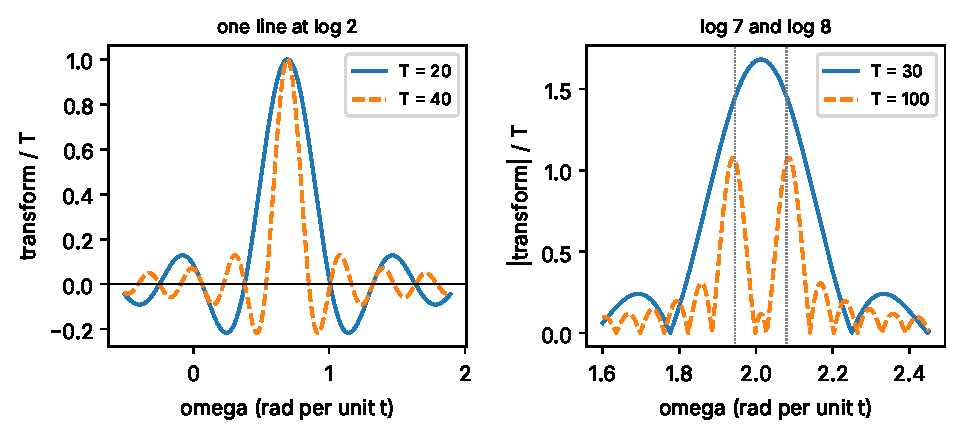
\includegraphics[width=0.95\linewidth]{figs/fourier-transform_sinc.pdf}
\caption{Left: the transform \eqref{eq:fourier-transform-sinc} of $e^{i\omega_0 t}$ observed for a window of length $T$, divided by $T$, with $\omega_0=\log2$. Doubling $T$ from 20 to 40 halves the width of the main lobe; the zeros sit at $\omega_0\pm2\pi k/T$. Right: two equal oscillations at $\log7=1.946$ and $\log8=2.079$, separated by $0.134$. With $T=30$ ($2\pi/T=0.209$) they merge into one peak; with $T=100$ ($2\pi/T=0.063$) they are resolved.}
\label{fig:fourier-transform-sinc}
\end{figure}

\subsection{The largest sidelobe}

Where are the sidelobe maxima? Differentiate with the quotient rule:
\begin{equation}
\frac{\dd}{\dd x}\frac{\sin x}{x}=\frac{x\cos x-\sin x}{x^2}.
\end{equation}
This vanishes when $x\cos x=\sin x$, i.e.\ $\tan x=x$. Besides $x=0$, the first positive solution lies between $\pi$ and $3\pi/2$; solving numerically (bisection or Brent, Chapter~\ref{ch:asymptotics}) gives $x=4.4934$, where $\abs{\mathrm{sinc}\,x}=0.2172$. So the tallest ripple of a finite-window sinusoid is about $22\%$ of the main peak in amplitude. Engineers quote this as $20\log_{10}0.2172=-13.3$ decibels.

\subsection{Real sinusoids}

A real oscillation $A\sin(\omega_0t)$ is a sum of two complex ones (Chapter~\ref{ch:complex}):
\[A\sin(\omega_0t)=\frac{A}{2i}e^{i\omega_0t}-\frac{A}{2i}e^{-i\omega_0t}.\]
By linearity (P1) and \eqref{eq:fourier-transform-sinc}, its windowed transform is
\begin{equation}
\frac{AT}{2i}\left[\mathrm{sinc}\!\left(\frac{(\omega-\omega_0)T}{2}\right)-\mathrm{sinc}\!\left(\frac{(\omega+\omega_0)T}{2}\right)\right].
\label{eq:fourier-transform-realsin}
\end{equation}
There are two peaks, at $+\omega_0$ and $-\omega_0$. At $\omega=\omega_0$ the first sinc equals 1 and the second is evaluated at $x=\omega_0T$, where $\abs{\mathrm{sinc}}\le1/(\omega_0 T)$. \emph{If} $\omega_0T\gg1$ (many cycles fit in the window), that second term is negligible and
\begin{equation}
\abs{\hat g(\omega_0)}\approx\frac{AT}{2}.
\label{eq:fourier-transform-AT2}
\end{equation}
For the prime-2 wave of RE2 with $T$ in the hundreds, $\omega_0T=T\log2$ is several hundred, so this condition is comfortably met.

\subsection{Resolution: when can two frequencies be told apart?}

Suppose the signal contains two oscillations of equal strength at $\omega_1$ and $\omega_2$. Each produces its own sinc peak. If they are far apart compared with the main-lobe half-width, you see two peaks. If they are much closer, the two humps merge into one. A conventional dividing line, the same one used for the resolving power of a telescope (the Rayleigh criterion in your physics course), is that the peak of one falls on the first zero of the other:
\begin{equation}
\boxed{\;\abs{\omega_2-\omega_1}\gtrsim\frac{2\pi}{T}\quad\text{(resolution of a window of length }T).}
\label{eq:fourier-transform-resolution}
\end{equation}
The quantity $2\pi/T$ is called the \textbf{Fourier resolution} of the window. The ``$\gtrsim$'' reminds you that the exact factor depends on the criterion chosen; what does not depend on any convention is the scaling $1/T$.

There is a second, more physical way to see \eqref{eq:fourier-transform-resolution}. Over the window, the phase of $e^{i\omega_2t}$ relative to $e^{i\omega_1t}$ changes by $(\omega_2-\omega_1)T$. In Chapter~\ref{ch:fourier-series} you met this as beats: the two oscillations drift in and out of step with beat period $2\pi/\abs{\omega_2-\omega_1}$. Unless the window contains about one full beat, you never see them drift apart. We can make this quantitative. For real $\theta$,
\[\abs{e^{i\theta}-1}=\abs{e^{i\theta/2}}\,\abs{e^{i\theta/2}-e^{-i\theta/2}}=2\abs{\sin(\theta/2)}\le\abs\theta,\]
using $\abs{\sin y}\le\abs y$. With $\theta=(\omega_2-\omega_1)t$,
\begin{equation}
\abs{e^{i\omega_2t}-e^{i\omega_1t}}=\abs{e^{i\omega_1t}}\,\abs{e^{i(\omega_2-\omega_1)t}-1}\le\abs{\omega_2-\omega_1}\,\abs t\le\abs{\omega_2-\omega_1}\frac T2
\label{eq:fourier-transform-indist}
\end{equation}
for every $t$ in the window $\abs t\le T/2$. If $\abs{\omega_2-\omega_1}T\ll1$, the two functions differ by a tiny amount everywhere in the window: no analysis of the windowed data, Fourier or otherwise, can tell them apart. The same inequality has a sobering consequence for prediction that Chapter~\ref{ch:sparse-frequency} develops: a frequency known only to within $\delta\omega$ gives a phase error $\delta\omega\,\Delta t$ at a distance $\Delta t$ outside the window, which grows the further you extrapolate.

\begin{sample}{Resolving prime-power frequencies}
The fluctuation of the zeros contains oscillations at angular frequencies $\log q$ for prime powers $q$ (Chapter~\ref{ch:explicit-formula}). (a) What window length $T$ is needed to resolve $\log8$ from $\log9$? (b) The paper's operator fits use zeros 1--400, which span heights from $t_1=14.13$ to $t_{400}\approx680$. Can that window resolve $\log 8$ from $\log 9$? Can it resolve $\log127$ from $\log128$?

\textbf{Step 1: Separations.} $\log9-\log8=\log(9/8)=0.1178$, and $\log128-\log127=\log(128/127)=0.00784$.

\textbf{Step 2: Required $T$} from \eqref{eq:fourier-transform-resolution}: $T\gtrsim2\pi/0.1178=53.3$ for the first pair and $T\gtrsim2\pi/0.00784=801$ for the second.

\textbf{Step 3: The paper's window.} We take the window length to be the distance between the first and last sample, $T=t_{400}-t_1\approx666$. (The paper does not spell out whether its $T$ is $t_{400}-t_1$ or $t_{400}$; the two differ by 2\%, which changes nothing below.) Then $2\pi/T\approx0.0094$.

\textbf{Step 4: Compare.} $0.1178\gg0.0094$, so $\log8$ and $\log9$ are resolved with room to spare. $0.00784<0.0094$, so $\log127$ and $\log128$ are not: within this window they look like a single frequency.

\[\boxed{T\gtrsim53.3\ \text{for }8/9;\quad T\gtrsim801\ \text{for }127/128;\quad\text{with }T\approx666:\ 8/9\text{ yes},\ 127/128\text{ no}.}\]
\end{sample}

\subsection{Lines and almost periodic functions}

For a function that oscillates forever, \eqref{eq:fourier-transform-sinc} suggests dividing by $T$: the peak value $T$ becomes 1 and the width $\to0$ as $T\to\infty$. This leads to the \emph{mean Fourier coefficient}
\begin{equation}
a(\omega)=\lim_{T\to\infty}\frac1T\int_0^Tf(t)\,e^{-i\omega t}\,\dd t ,
\label{eq:fourier-transform-mean}
\end{equation}
which is the right spectral notion for the almost periodic sums of Chapter~\ref{ch:fourier-series} (the theory of such functions is due to Harald Bohr).

Let $f(t)=\sum_{j=1}^{J}b_je^{i\lambda_jt}$ be a finite sum with distinct real frequencies $\lambda_j$ and complex amplitudes $b_j$. By linearity, \eqref{eq:fourier-transform-mean} needs only $\frac1T\int_0^Te^{i(\lambda_j-\omega)t}\,\dd t$. If $\lambda_j=\omega$ the integrand is 1 and the result is 1. If $\lambda_j\neq\omega$,
\[\frac1T\int_0^Te^{i(\lambda_j-\omega)t}\,\dd t=\frac{e^{i(\lambda_j-\omega)T}-1}{i(\lambda_j-\omega)T},\qquad
\left|\,\cdot\,\right|\le\frac{2}{\abs{\lambda_j-\omega}\,T}\to0,\]
because $\abs{e^{i\theta}-1}\le2$. Therefore
\begin{equation}
a(\omega)=\begin{cases}b_j,&\omega=\lambda_j,\\0,&\omega\text{ not among the }\lambda_j.\end{cases}
\label{eq:fourier-transform-lines}
\end{equation}
The spectrum of an almost periodic sum consists of isolated \emph{lines}, whether or not the frequencies share a period. For a real term $A\sin(\lambda t)=\frac{A}{2i}e^{i\lambda t}-\frac{A}{2i}e^{-i\lambda t}$ the lines sit at $\pm\lambda$ with $\abs{a}=\abs A/2$.

\textbf{Applied to RE2, the prime-2 wave} $-\frac1\pi\sum_{m=1}^{3}\frac{\sin(mt\log2)}{m2^{m/2}}$: the amplitudes $\abs{A_m}=1/(\pi m2^{m/2})$ are $0.2251$, $0.0796$ and $0.0375$ for $m=1,2,3$, so the lines at $m\log2$ have $\abs a=0.1125$, $0.0398$ and $0.0188$. The longest period is $2\pi/\log 2\approx9.065$ in $t$.

\textbf{Applied to the paper's Eq.~(4)}: $N_{\rm fl}(t)=-\frac1\pi\sum_{p}\sum_{m=1}^{3}\frac{\sin(mt\log p)}{mp^{m/2}}$, with $p$ running over a set of primes (an integer greater than 1 divisible only by 1 and itself) and $\log$ the natural logarithm. Its spectrum is a set of lines at $\omega=\pm m\log p=\pm\log(p^m)$ with $\abs a=1/(2\pi mp^{m/2})$. These frequencies are all different: $m\log p=k\log q$ would mean $p^m=q^k$, which by the unique factorization of integers (Chapter~\ref{ch:primes}) forces $p=q$ and $m=k$. Through a window of length $T$, each line becomes a sinc of height $\approx T\abs a$ and width $\sim2\pi/T$.

\subsection{Leakage and tapered windows}

Look again at \cref{fig:fourier-transform-sinc}: the ripples of a strong line spill into frequencies where nothing is actually present. This is \textbf{spectral leakage}. A weak line sitting under a sidelobe of a strong one can be hidden, or a sidelobe can be mistaken for a weak line. The culprit is the abrupt switch-on and switch-off of the box: sharp edges in $t$ need many frequencies to build.

A \emph{tapered} window rises and falls smoothly. The most common is the \textbf{Hann window}, on $\abs t\le T/2$,
\begin{equation}
w(t)=\tfrac12\bigl(1+\cos(2\pi t/T)\bigr)=\tfrac12+\tfrac14e^{i2\pi t/T}+\tfrac14e^{-i2\pi t/T},
\end{equation}
which is 1 at the center and falls to 0 at the edges. Its transform follows from linearity and modulation applied to the box transform $B(\omega)=2\sin(\omega T/2)/\omega$:
\begin{equation}
\hat w(\omega)=\tfrac12B(\omega)+\tfrac14B\!\left(\omega-\tfrac{2\pi}T\right)+\tfrac14B\!\left(\omega+\tfrac{2\pi}T\right).
\end{equation}
Measure frequency in \emph{bins}, $\delta=\omega T/(2\pi)$, so one bin is one Fourier resolution. Then $B=T\,s(\delta)$ with $s(\delta)=\sin(\pi\delta)/(\pi\delta)$, and
\begin{equation}
\frac{\hat w}{T}=\tfrac12s(\delta)+\tfrac14s(\delta-1)+\tfrac14s(\delta+1).
\label{eq:fourier-transform-hann3}
\end{equation}
We can simplify. Since $\sin(\pi\delta\pm\pi)=-\sin(\pi\delta)$, $s(\delta\pm1)=-\sin(\pi\delta)/(\pi(\delta\pm1))$. Factor out $\sin(\pi\delta)/\pi$:
\begin{align}
\frac{\hat w}{T}&=\frac{\sin\pi\delta}{\pi}\left[\frac{1}{2\delta}-\frac{1}{4(\delta-1)}-\frac{1}{4(\delta+1)}\right]\notag\\
&=\frac{\sin\pi\delta}{\pi}\left[\frac{1}{2\delta}-\frac{2\delta}{4(\delta^2-1)}\right]\quad\text{(common denominator of last two)}\notag\\
&=\frac{\sin\pi\delta}{\pi}\cdot\frac{(\delta^2-1)-\delta^2}{2\delta(\delta^2-1)}\notag\\
&=-\frac{\sin\pi\delta}{2\pi\delta(\delta^2-1)}.
\label{eq:fourier-transform-hann}
\end{align}
Three consequences, plotted in \cref{fig:fourier-transform-leakage}:
\begin{itemize}
\item \textbf{Peak.} As $\delta\to0$, $\sin(\pi\delta)/(\pi\delta)\to1$ and the formula gives $-1/(2\cdot(-1))=\tfrac12$: the peak is $T/2$ (the Hann window has half the area of the box).
\item \textbf{Wider main lobe.} At $\delta=\pm1$ the numerator and the factor $\delta^2-1$ both vanish, and the limit is $\tfrac14$, not 0 (Problem~10). The first zeros are at $\delta=\pm2$: the main lobe is twice as wide as for the box.
\item \textbf{Much lower sidelobes.} For large $\abs\delta$ the size falls like $1/\abs\delta^3$ instead of $1/\abs\delta$. The highest Hann sidelobe, divided by the Hann peak value $\tfrac12$, is $0.0267$ ($-31.5$ dB). The corresponding box figure is $0.217$, divided by the box peak value 1.
\end{itemize}

\begin{figure}[htbp]\centering
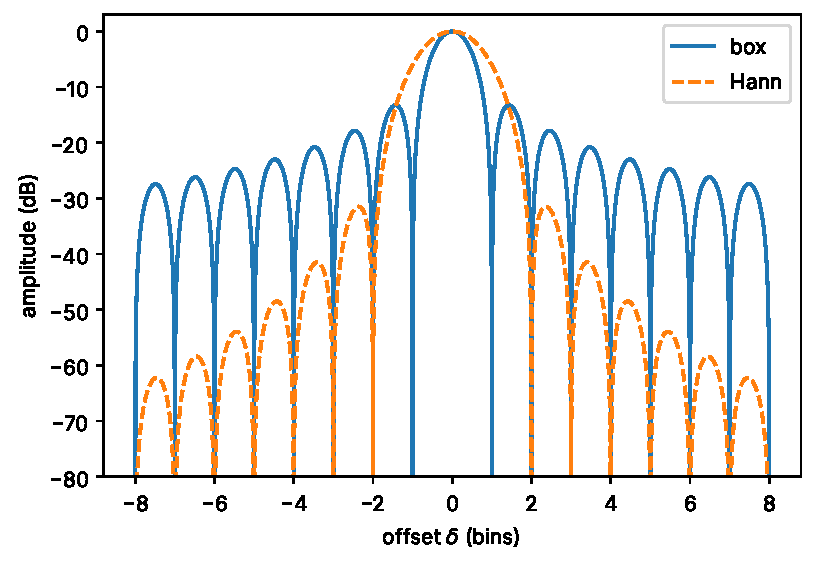
\includegraphics[width=0.85\linewidth]{figs/fourier-transform_leakage.pdf}
\caption{Leakage: the amplitude spectrum of a single line seen through a rectangular window (box) and through a Hann window, each normalized to its own peak and shown in decibels ($20\log_{10}$ of the amplitude ratio). The horizontal axis is the offset from the line in bins, $\delta=(\omega-\omega_0)T/2\pi$. The Hann main lobe is twice as wide, but its sidelobes are far lower and decay much faster.}
\label{fig:fourier-transform-leakage}
\end{figure}

\begin{sample}{How much of a peak do you see if you miss it by half a bin?}
You compute a windowed spectrum only at frequencies spaced one bin ($2\pi/T$) apart, and a line happens to lie exactly halfway between two of them. What fraction of the true peak amplitude do you see with the box and with the Hann window?

\textbf{Step 1: Box.} The offset is $\delta=\tfrac12$, so the ratio to the peak is $s(\tfrac12)=\sin(\pi/2)/(\pi/2)=2/\pi=0.6366$.

\textbf{Step 2: Hann.} From \eqref{eq:fourier-transform-hann} at $\delta=\tfrac12$: $-\sin(\pi/2)/(2\pi\cdot\tfrac12\cdot(\tfrac14-1))=1/(0.75\pi)=0.4244$. Divide by the Hann peak $\tfrac12$: $8/(3\pi)=0.8488$.

\[\boxed{\text{box: }2/\pi=0.637;\qquad\text{Hann: }8/(3\pi)=0.849.}\]
\end{sample}
The loss is called ``scalloping''. The cure, whichever window you use, is to evaluate the spectrum on a grid finer than one bin; Section~\ref{sec:fourier-transform-periodogram} returns to this.

\begin{pitfall}
A tapered window does \emph{not} improve resolution. Only a longer $T$ does. Tapering trades a wider main lobe (worse at separating two close lines of equal strength) for lower sidelobes (better at seeing a weak line far from a strong one). Choose the window for the question you are asking.
\end{pitfall}

\begin{checkpoint}
You double the length $T$ of the window through which you observe $e^{i\omega_0t}$. What happens to the height of the peak of $\abs{\hat g}$, to the width of its main lobe, and to the height of the peak of $\abs{\hat g}/T$?
\end{checkpoint}
\checkanswer{The peak height $T$ doubles, the main-lobe width $4\pi/T$ halves, and $\abs{\hat g}/T$ still peaks at 1.}

\begin{keyideas}

\item A finite window of length $T$ turns each line at $\omega_0$ into $T\,\mathrm{sinc}((\omega-\omega_0)T/2)$, Eq.~\eqref{eq:fourier-transform-sinc}: main lobe from $\omega_0-2\pi/T$ to $\omega_0+2\pi/T$, largest sidelobe $0.217$ of the peak.
\item Two frequencies are resolved when $\abs{\Delta\omega}\gtrsim2\pi/T$, the Fourier resolution, Eq.~\eqref{eq:fourier-transform-resolution}; when $\abs{\Delta\omega}T\ll1$ they are indistinguishable in the window, Eq.~\eqref{eq:fourier-transform-indist}.
\item An almost periodic sum has a line spectrum, Eq.~\eqref{eq:fourier-transform-lines}; the explicit-formula fluctuation has lines at $\log p^m$ of size $1/(2\pi mp^{m/2})$.
\item Leakage comes from the window's sidelobes; the Hann window, Eq.~\eqref{eq:fourier-transform-hann}, lowers them at the price of a doubled main lobe.

\end{keyideas}

%======================================================================
\section{Sampling: uniform, irregular and aliasing}\label{sec:fourier-transform-sampling}
% DYK-BEGIN
\begin{didyouknow}{Why CDs Use 44.1 kHz}
Human hearing tops out near 20 kHz. To capture a signal without aliasing you must sample faster than twice its highest frequency, so audio CDs sample 44{,}100 times per second, just above $2\times20$ kHz. Aliasing shows up in films too. A spinning wagon wheel filmed at 24 frames per second can appear to turn slowly backward.
\end{didyouknow}
% DYK-END

A computer never holds a function $f(t)$ for all $t$; it holds a list of values $y_j=f(t_j)$ at sample points $t_j$. For an oscilloscope the $t_j$ are equally spaced. For the Riemann zeros the ``samples'' are the zeros themselves, and they are not equally spaced. Both cases matter to us.

\subsection{Uniform samples and aliasing}

Let $t_j=j\,\Delta t$ for $j=0,1,\dots,N-1$, so the samples span a window of length about $T=N\Delta t$. The natural approximation to the windowed transform is the Riemann sum
\begin{equation}
\int_0^Tf(t)e^{-i\omega t}\,\dd t\approx\Delta t\sum_{j=0}^{N-1}f(t_j)\,e^{-i\omega t_j}.
\label{eq:fourier-transform-riemannsum}
\end{equation}
Something new happens on the right side. Replace $\omega$ by $\omega+2\pi/\Delta t$:
\[e^{-i(\omega+2\pi/\Delta t)j\Delta t}=e^{-i\omega j\Delta t}\,e^{-2\pi ij}=e^{-i\omega j\Delta t},\]
since $e^{-2\pi ij}=1$ for every integer $j$. So the sampled sum is periodic in $\omega$ with period $2\pi/\Delta t$. Equivalently, the two oscillations $e^{i\omega t}$ and $e^{i(\omega+2\pi/\Delta t)t}$ have \emph{identical samples}: from the samples alone they cannot be distinguished. This is \textbf{aliasing}. For real signals, (P2) adds a mirror symmetry, so $\omega$ is also confused with $2\pi/\Delta t-\omega$. All distinct information lives in
\begin{equation}
0\le\omega\le\omega_{\rm N}=\frac{\pi}{\Delta t},
\label{eq:fourier-transform-nyquist}
\end{equation}
where $\omega_{\rm N}$ is the \textbf{Nyquist frequency}: half the sampling rate, or ``two samples per cycle''. A component above $\omega_{\rm N}$ does not disappear; it masquerades as one below. You have seen this in films where a fast-spinning wagon wheel appears to turn slowly backwards: the camera samples at a fixed rate.

\begin{beyond}
\textbf{Taken on trust: the sampling theorem.} If $\hat f(\omega)=0$ for all $\abs\omega>\omega_{\rm N}$ (a ``band-limited'' signal), then $f$ is determined at every $t$ by its uniform samples at spacing $\Delta t=\pi/\omega_{\rm N}$. This is the Shannon (or Nyquist--Shannon) sampling theorem; a practical discussion is in \cite{nr}. We will not need it, only the aliasing identity above, which we have proved.
\end{beyond}

\begin{figure}[htbp]\centering
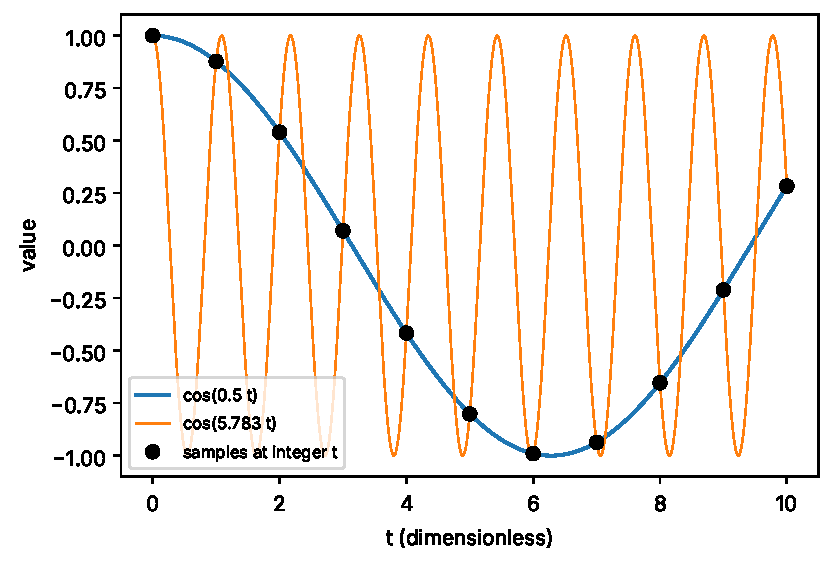
\includegraphics[width=0.85\linewidth]{figs/fourier-transform_aliasing.pdf}
\caption{Aliasing. The slow oscillation $\cos(0.5t)$ and the fast one $\cos((2\pi-0.5)t)=\cos(5.783t)$ pass through exactly the same values at the integer sample times $t=0,1,2,\dots$ (dots). With $\Delta t=1$ the Nyquist frequency is $\pi$, and $5.783$ lies above it.}
\label{fig:fourier-transform-aliasing}
\end{figure}

\begin{sample}{An alias, and the ``Nyquist frequency'' of the zeros}
(a) With $\Delta t=1$, show that $\cos(0.5t)$ and $\cos(5.7832\,t)$ have the same samples. (b) Near zero number $n=400$, the zeros are spaced on average by the mean gap $\mathrm{gap}_n=2\pi/\log(s_n/2\pi)$, where $s_n$ is the smooth zero of Chapter~\ref{ch:counting-zeros} (the solution of $N_{\rm sm}(s_n)=n-\tfrac12$, paper Eq.~(1)). If the zeros were equally spaced at this gap, what would their Nyquist frequency be?

\textbf{Step 1: The alias.} $5.7832=2\pi-0.5$ to the digits shown. At $t=j$, $\cos((2\pi-0.5)j)=\cos(2\pi j)\cos(0.5j)+\sin(2\pi j)\sin(0.5j)=\cos(0.5j)$, using $\cos(2\pi j)=1$ and $\sin(2\pi j)=0$.

\textbf{Step 2: Smooth zero and gap.} Solving $N_{\rm sm}(s)=399.5$ numerically gives $s_{400}=679.9$; then $\log(s_{400}/2\pi)=4.684$ and $\mathrm{gap}_{400}=2\pi/4.684=1.341$.

\textbf{Step 3: Equivalent Nyquist frequency.} $\omega_{\rm N}=\pi/\mathrm{gap}=\tfrac12\log(s_{400}/2\pi)=2.342$.

\[\boxed{\cos(5.7832\,j)=\cos(0.5\,j);\qquad \pi/\mathrm{gap}_{400}=\tfrac12\log(s_{400}/2\pi)\approx2.34.}\]
\end{sample}

The neat form $\pi/\mathrm{gap}_n=\tfrac12\log(s_n/2\pi)$ shows that the zeros sample more densely as you go higher, so this ``equivalent Nyquist frequency'' slowly rises with height. But the zeros are \emph{not} equally spaced, and that changes the story, as we now see.

\subsection{Irregular samples and the spectral window}

When the $t_j$ are irregular, no FFT shortcut applies (Section~\ref{sec:fourier-transform-dft}), but nothing stops us from computing the sum directly:
\begin{equation}
F(\omega)=\sum_{j=1}^{N}y_j\,e^{-i\omega t_j}.
\label{eq:fourier-transform-directsum}
\end{equation}
This is sometimes called a nonuniform discrete Fourier transform. Its cost is $N$ complex exponentials per frequency; for $N=1000$ zeros and $10^4$ trial frequencies that is $10^7$ operations, a fraction of a second on a laptop. For real data $y_j$, $F(-\omega)=\overline{F(\omega)}$ by the same argument as (P2).

What does \eqref{eq:fourier-transform-directsum} do to a single oscillation? Put $y_j=b\,e^{i\omega_0t_j}$:
\begin{equation}
F(\omega)=b\sum_{j}e^{-i(\omega-\omega_0)t_j}=b\,W(\omega-\omega_0),\qquad W(\omega)=\sum_{j=1}^{N}e^{-i\omega t_j}.
\label{eq:fourier-transform-specwin}
\end{equation}
The function $W$ is the \textbf{spectral window} of the sampling pattern: it plays for sampled data the role the sinc played for the continuous window. It depends only on \emph{where} you sampled, not on the data. Always $W(0)=N$.

\emph{Uniform case.} With $t_j=j\Delta t$, $j=0,\dots,N-1$, $W$ is a geometric series with ratio $r=e^{-i\omega\Delta t}$ (Chapter~\ref{ch:series}). For $r\ne1$,
\begin{align}
W(\omega)&=\frac{1-r^N}{1-r}=\frac{1-e^{-iN\omega\Delta t}}{1-e^{-i\omega\Delta t}}.\notag
\end{align}
Write $1-e^{-i\theta}=e^{-i\theta/2}(e^{i\theta/2}-e^{-i\theta/2})=2i\,e^{-i\theta/2}\sin(\theta/2)$ for numerator ($\theta=N\omega\Delta t$) and denominator ($\theta=\omega\Delta t$). The factors $2i$ cancel, the exponentials have modulus 1, and
\begin{equation}
\abs{W(\omega)}=\left|\frac{\sin(N\omega\Delta t/2)}{\sin(\omega\Delta t/2)}\right| .
\label{eq:fourier-transform-dirichlet}
\end{equation}
This ratio of sines is called the \textbf{Dirichlet kernel}. For small $\omega\Delta t$, $\sin(\omega\Delta t/2)\approx\omega\Delta t/2$ and \eqref{eq:fourier-transform-dirichlet} becomes $\abs{2\sin(\omega T/2)/\omega}/\Delta t$ with $T=N\Delta t$: the box transform, as the Riemann sum \eqref{eq:fourier-transform-riemannsum} promised. But the denominator also vanishes at $\omega=2\pi k/\Delta t$, where $\abs W$ climbs back to $N$: those repeated full-height peaks \emph{are} aliasing.

\emph{Irregular case.} For $\abs{W(\Omega)}$ to equal $N$ again at some $\Omega\ne0$, all the unit arrows $e^{-i\Omega t_j}$ would have to point the same way (only then is the triangle inequality an equality). So all the phases $\Omega t_j$ would have to agree up to multiples of $2\pi$; that is, every difference $\Omega(t_j-t_l)$ would have to be a multiple of $2\pi$. Generic irregular points do not allow this. So exact aliasing disappears. What remains is a ``floor'' of partial cancellations. Its typical size follows from a heuristic count. Expanding the modulus squared, $\abs{W(\Omega)}^2=\sum_j\sum_l e^{-i\Omega(t_j-t_l)}$. The $N$ terms with $j=l$ each equal 1. For points scattered at random, the remaining $N(N-1)$ terms are unit arrows pointing in all directions, and they largely cancel. If their total were negligible, we would have $\abs{W}^2\approx N$, that is, $\abs W\approx\sqrt N$. This is a heuristic, not a proof; Chapter~\ref{ch:probability} supplies the language of averages needed to make it precise. It shows that the floor lies well below the central peak $N$ for large $N$. In principle, then, irregular samples can reveal frequencies above the ``equivalent Nyquist'' value $\pi/\overline{\Delta t}$. Section~\ref{sec:fourier-transform-paper} describes a result of the paper that is compatible with this (frequencies recovered above the equivalent Nyquist value), though the mechanism is not established.

Two warnings specific to the zeros. First, irregular sampling also \emph{weights} the data: regions with more samples count more in \eqref{eq:fourier-transform-directsum}. The zeros become denser with height; their average number per unit $t$ is $\frac{1}{2\pi}\log\frac{t}{2\pi}$ (we derive this in Section~\ref{sec:fourier-transform-landau}), about $0.13$ at $t_1$ and about $0.75$ at $t_{400}$. Sampling at the zeros therefore acts like a window that rises across the data range. Second, the zeros are not random points at all: their spectral window $W$ has sharp spikes at the logarithms of prime powers (Section~\ref{sec:fourier-transform-landau}). A sampling pattern with its own structure can imprint that structure on any spectrum computed from it.

\begin{checkpoint}
You sample a signal every $\Delta t=0.1$. What is the Nyquist frequency? A component at $\omega=40$ is present; at what frequency in $[0,\omega_{\rm N}]$ does it appear?
\end{checkpoint}
\checkanswer{$\omega_{\rm N}=\pi/0.1=31.4$. The alias period is $2\pi/\Delta t=62.83$, so $40$ is confused with $62.83-40=22.83$, which lies below the Nyquist frequency.}

\begin{keyideas}

\item Uniform samples at spacing $\Delta t$ cannot distinguish $\omega$ from $\omega+2\pi/\Delta t$ (aliasing); real signals are fully described on $0\le\omega\le\pi/\Delta t$, Eq.~\eqref{eq:fourier-transform-nyquist}.
\item For irregular samples compute the direct sum $F(\omega)=\sum y_je^{-i\omega t_j}$, Eq.~\eqref{eq:fourier-transform-directsum}; a sampled oscillation produces the spectral window $W(\omega-\omega_0)$, Eq.~\eqref{eq:fourier-transform-specwin}.
\item The uniform spectral window is the Dirichlet kernel \eqref{eq:fourier-transform-dirichlet}, with full-height aliases; irregular sampling removes exact aliases but weights the data by sample density, and for the zeros the window itself has structure.

\end{keyideas}

%======================================================================
\section{The discrete Fourier transform and the FFT}\label{sec:fourier-transform-dft}

For uniformly sampled data there is a special set of frequencies at which the sum \eqref{eq:fourier-transform-directsum} has beautiful properties and can be computed astonishingly fast.

\subsection{Definition and inverse}

Given $N$ numbers $x_0,x_1,\dots,x_{N-1}$ (real or complex), their \textbf{discrete Fourier transform} (DFT) is the list of $N$ numbers
\begin{equation}
X_k=\sum_{j=0}^{N-1}x_j\,e^{-2\pi ijk/N},\qquad k=0,1,\dots,N-1.
\label{eq:fourier-transform-dft}
\end{equation}
If $x_j=f(j\Delta t)$, then $X_k$ is the sum \eqref{eq:fourier-transform-directsum} evaluated at
\begin{equation}
\omega_k=\frac{2\pi k}{N\Delta t}=k\,\frac{2\pi}{T},\qquad T=N\Delta t,
\end{equation}
because $\omega_kt_j=2\pi kj/N$. So the DFT samples the spectrum exactly once per Fourier resolution, one value per bin. Indices $k>N/2$ are aliases of negative frequencies: $e^{-2\pi ijk/N}=e^{-2\pi ij(k-N)/N}$ since $e^{2\pi ij}=1$.

The key fact is an orthogonality relation, a discrete cousin of the orthogonality of $e^{ik\omega t}$ in Chapter~\ref{ch:fourier-series}. For an integer $m$,
\begin{equation}
\sum_{k=0}^{N-1}e^{2\pi ikm/N}=\begin{cases}N,&m\text{ a multiple of }N,\\0,&\text{otherwise.}\end{cases}
\label{eq:fourier-transform-orth}
\end{equation}
\emph{Proof.} If $m$ is a multiple of $N$, every term is $e^{2\pi i\times\text{integer}}=1$, and there are $N$ terms. Otherwise the ratio $r=e^{2\pi im/N}\ne1$, and the geometric series gives $(1-r^N)/(1-r)$ with $r^N=e^{2\pi im}=1$, so the sum is $0$. $\square$

\textbf{Inverse DFT.} Multiply \eqref{eq:fourier-transform-dft} by $e^{2\pi ilk/N}$, for a fixed index $l$, and sum over $k$:
\begin{align}
\sum_{k=0}^{N-1}X_ke^{2\pi ilk/N}&=\sum_{k}\sum_{j}x_je^{-2\pi ijk/N}e^{2\pi ilk/N}\notag\\
&=\sum_{j}x_j\sum_{k}e^{2\pi ik(l-j)/N}\quad\text{(swap finite sums)}\notag\\
&=\sum_jx_j\,N\,[j=l]\quad\text{(by \eqref{eq:fourier-transform-orth}; }l-j\text{ is a multiple of }N\text{ only if }j=l)\notag\\
&=Nx_l .\notag
\end{align}
Here $[j=l]$ is 1 if $j=l$ and 0 otherwise. Hence
\begin{equation}
x_l=\frac1N\sum_{k=0}^{N-1}X_k\,e^{2\pi ilk/N}.
\label{eq:fourier-transform-idft}
\end{equation}
Unlike the continuous case, this inversion is fully proved, with no conditions: $N$ numbers in, $N$ numbers out, nothing lost.

\textbf{Real data.} If all $x_j$ are real, conjugating \eqref{eq:fourier-transform-dft} gives $\overline{X_k}=\sum x_je^{2\pi ijk/N}=\sum x_je^{-2\pi ij(N-k)/N}=X_{N-k}$, using $e^{-2\pi ijN/N}=1$. So
\begin{equation}
X_{N-k}=\overline{X_k}\qquad(x\text{ real}),
\label{eq:fourier-transform-dftsym}
\end{equation}
and in particular $X_0=\sum x_j$ is real, and if $N$ is even, $X_{N/2}=\sum x_j(-1)^j$ is real. Only about half the coefficients are independent; \texttt{numpy.fft.rfft} returns exactly those, $X_0,\dots,X_{\lfloor N/2\rfloor}$.

\textbf{Parseval for the DFT.} We prove in Section~\ref{sec:fourier-transform-wk} that
\begin{equation}
\sum_{j=0}^{N-1}\abs{x_j}^2=\frac1N\sum_{k=0}^{N-1}\abs{X_k}^2,
\label{eq:fourier-transform-parseval}
\end{equation}
the discrete form of Parseval's relation of Chapter~\ref{ch:fourier-series}.

\begin{sample}{A DFT by hand}
Compute the DFT of $x=(2,1,0,1)$ and verify Parseval's relation \eqref{eq:fourier-transform-parseval}.

\textbf{Step 1: The phases.} With $N=4$, $e^{-2\pi ijk/4}=(e^{-i\pi/2})^{jk}=(-i)^{jk}$. The powers of $-i$ are $1,-i,-1,i,1,\dots$

\textbf{Step 2: Each coefficient.}
\begin{align*}
X_0&=2+1+0+1=4,\\
X_1&=2+1(-i)+0+1(-i)^3=2-i+i=2,\\
X_2&=2+1(-i)^2+0+1(-i)^6=2-1-1=0,\\
X_3&=2+1(-i)^3+0+1(-i)^9=2+i-i=2.
\end{align*}
Note $X_3=\overline{X_1}$, as \eqref{eq:fourier-transform-dftsym} requires.

\textbf{Step 3: Parseval.} Left side: $4+1+0+1=6$. Right side: $(16+4+0+4)/4=6$.

\textbf{Step 4: Interpret.} $x_j=1+\cos(\pi j/2)$, a constant plus one cosine that completes one cycle in four samples; the DFT finds the constant in $X_0$ and the cosine in $X_1$ and its mirror $X_3$.

\[\boxed{X=(4,2,0,2),\qquad\textstyle\sum\abs{x_j}^2=6=\frac14\sum\abs{X_k}^2.}\]
\end{sample}

\begin{pycode}
import numpy as np

x = np.array([2.0, 1.0, 0.0, 1.0])
N = len(x)
idx = np.arange(N)                    # sample indices 0..N-1
# the DFT straight from the definition; 2j is Python for 2i
X_def = np.array([np.sum(x*np.exp(-2j*np.pi*idx*k/N)) for k in range(N)])
X_fft = np.fft.fft(x)                 # numpy uses the same sign convention
print(np.round(X_def, 12))            # [4, 2, 0, 2]
print(np.allclose(X_def, X_fft))      # True
print(np.sum(x**2), np.sum(np.abs(X_fft)**2)/N)   # 6.0 6.0 (Parseval)
print(np.fft.rfft(x))                 # the independent half: X_0, X_1, X_2
\end{pycode}

\begin{pitfall}
Different books and libraries put the $1/N$ in different places (in front of the forward sum, the inverse sum, or $1/\sqrt N$ on both) and some use $e^{+2\pi ijk/N}$ in the forward direction. \texttt{numpy.fft.fft} uses exactly Eq.~\eqref{eq:fourier-transform-dft} with no factor in front, and \texttt{numpy.fft.ifft} includes the $1/N$. Peak \emph{positions} never depend on the convention; peak \emph{heights} do, so always check before comparing numbers.
\end{pitfall}

\subsection{The fast Fourier transform}

Computing all $N$ coefficients of \eqref{eq:fourier-transform-dft} directly takes $N$ multiplications each, $N^2$ in total. The \textbf{fast Fourier transform} (FFT) does the same job in about $N\log_2N$ operations when $N$ is a power of 2. Here is the whole idea.

Write $w=e^{-2\pi i/N}$, so $X_k=\sum_jx_jw^{jk}$. Split the sum into even $j=2l$ and odd $j=2l+1$ indices, $l=0,\dots,N/2-1$:
\begin{align}
X_k&=\sum_{l}x_{2l}w^{2lk}+\sum_lx_{2l+1}w^{(2l+1)k}\notag\\
&=\sum_lx_{2l}(w^2)^{lk}+w^k\sum_lx_{2l+1}(w^2)^{lk}.
\end{align}
Now $w^2=e^{-2\pi i/(N/2)}$ is exactly the ``$w$'' of a DFT of length $N/2$. So $X_k=E_k+w^kO_k$, where $E_k$ and $O_k$ are the length-$N/2$ DFTs of the even-indexed and odd-indexed samples. These have period $N/2$ in $k$, and $w^{N/2}=e^{-i\pi}=-1$, so for $k=0,\dots,N/2-1$,
\begin{equation}
X_k=E_k+w^kO_k,\qquad X_{k+N/2}=E_k-w^kO_k .
\label{eq:fourier-transform-butterfly}
\end{equation}
Two half-size DFTs plus $N$ simple combinations give the full DFT. Apply the same split to each half, and so on down to DFTs of length 1 (which are just $X_0=x_0$). If $C(N)$ is the operation count, $C(N)=2C(N/2)+N$ and $C(1)=0$. Divide by $N$: $C(N)/N=C(N/2)/(N/2)+1$. With $N=2^q$, applying this $q$ times gives $C(N)/N=C(1)/1+q=q$, so
\begin{equation}
C(N)=N\log_2N .
\end{equation}
(Algorithms of the same speed exist for $N$ that are not powers of 2; libraries handle this for you.)

\begin{sample}{Bins, Nyquist and the FFT saving}
You record $N=1024$ uniform samples at $\Delta t=0.5$. Find the bin spacing of the DFT, the Nyquist frequency, and the ratio of the direct cost $N^2$ to the FFT cost $N\log_2N$.

\textbf{Step 1: Window.} $T=N\Delta t=512$.

\textbf{Step 2: Bin spacing.} $\omega_{k+1}-\omega_k=2\pi/T=2\pi/512=0.01227$.

\textbf{Step 3: Nyquist.} $\omega_{\rm N}=\pi/\Delta t=2\pi=6.283$; equivalently the bin $k=N/2=512$.

\textbf{Step 4: Saving.} $N^2/(N\log_2N)=N/\log_2N=1024/10=102.4$.

\[\boxed{\Delta\omega=0.01227,\quad\omega_{\rm N}=6.283,\quad\text{FFT about }102\text{ times faster}.}\]
\end{sample}

\begin{pitfall}
The FFT needs \emph{uniform} sampling. The Riemann zeros are irregular in $t$, so a spectrum of the zeros in the frequency $\omega$ of $t$ must be computed as the direct sum \eqref{eq:fourier-transform-directsum}. But a sequence \emph{indexed by $n$}, such as the fluctuation $d_n$ of the $n$-th zero, is uniform in $n$, and the FFT applies to it perfectly well. Keep track of which variable your frequencies refer to: radians per unit of $t$, or radians per level.
\end{pitfall}

\begin{keyideas}

\item The DFT \eqref{eq:fourier-transform-dft} samples the spectrum once per bin $2\pi/T$; its inverse \eqref{eq:fourier-transform-idft} follows from the orthogonality \eqref{eq:fourier-transform-orth}.
\item For real data $X_{N-k}=\overline{X_k}$; only $X_0,\dots,X_{\lfloor N/2\rfloor}$ are independent.
\item The FFT splits even and odd samples, Eq.~\eqref{eq:fourier-transform-butterfly}, and costs $N\log_2N$ instead of $N^2$; it requires uniform sampling.

\end{keyideas}

%======================================================================
\section{The periodogram and finding peaks}\label{sec:fourier-transform-periodogram}

We now have the tools to answer, with real data, the question ``which frequencies are present, and how strongly?''

\subsection{Definition}

For samples $y_j$ at points $t_j$, $j=1,\dots,N$ (uniform or not), the \textbf{periodogram} is
\begin{equation}
P(\omega)=\frac1N\Bigl|\sum_{j=1}^{N}y_j\,e^{-i\omega t_j}\Bigr|^2=\frac{\abs{F(\omega)}^2}{N}.
\label{eq:fourier-transform-periodogram}
\end{equation}
For uniform samples at the DFT frequencies it is $P_k=\abs{X_k}^2/N$. It is a function of $\omega$ that you can evaluate on any grid you like. Because $P(-\omega)=P(\omega)$ for real data, we plot only $\omega>0$. Before computing it, subtract the mean of the $y_j$: otherwise the line at $\omega=0$, of height $N\bar y^2$, leaks into everything near $\omega=0$.

\subsection{How tall is a line, and how tall is the noise?}

\emph{A line.} Let $y_j=A\sin(\omega_0t_j)=\frac{A}{2i}(e^{i\omega_0t_j}-e^{-i\omega_0t_j})$. Then
\begin{equation}
F(\omega_0)=\frac{A}{2i}\Bigl(\sum_j1-\sum_je^{-2i\omega_0t_j}\Bigr)=\frac{A}{2i}\bigl(N-W(2\omega_0)\bigr),
\end{equation}
with $W$ the spectral window \eqref{eq:fourier-transform-specwin}. \emph{If} $\abs{W(2\omega_0)}\ll N$ (the analogue of $\omega_0T\gg1$ for a continuous window), then $\abs{F(\omega_0)}\approx NA/2$ and
\begin{equation}
P(\omega_0)\approx\frac{NA^2}{4}.
\label{eq:fourier-transform-lineheight}
\end{equation}
The line height grows in proportion to the number of samples.

\emph{Noise.} Now let $y_j=\varepsilon_j$ be ``noise'': values that are independent of one another, average zero, and have average square $\sigma^2$. (Chapter~\ref{ch:probability} defines these notions properly; here we use them informally.) Expanding the modulus squared,
\begin{equation}
\abs{F(\omega)}^2=\sum_{j}\sum_{l}\varepsilon_j\varepsilon_l\,e^{-i\omega(t_j-t_l)} .
\end{equation}
Average over many realizations of the noise. The terms with $j\neq l$ average to zero, because $\varepsilon_j$ and $\varepsilon_l$ are independent with average zero. The $N$ terms with $j=l$ each average to $\sigma^2$, and their phase factor is $e^0=1$. So the average of $\abs F^2$ is $N\sigma^2$, and the average periodogram is
\begin{equation}
\langle P(\omega)\rangle=\sigma^2,
\label{eq:fourier-transform-noise}
\end{equation}
independent of $N$ and of $\omega$ (``white'' noise). This is a heuristic result: a single realization fluctuates about this average by an amount of the same order. Putting \eqref{eq:fourier-transform-lineheight} and \eqref{eq:fourier-transform-noise} together, the line stands above the noise by a factor
\begin{equation}
\frac{P(\omega_0)}{\langle P\rangle}\approx\frac{NA^2}{4\sigma^2},
\label{eq:fourier-transform-snr}
\end{equation}
which grows with $N$. Longer data make lines stand out, however weak.

\begin{sample}{Detecting a weak oscillation}
A sinusoid of amplitude $A=0.1$ is buried in noise whose root-mean-square size $\sigma=0.3$ (the square root of the average of the squared noise values) is three times the sinusoid's amplitude. With $N=400$ samples, how much does its periodogram peak rise above the average noise level? From the peak, how would you estimate $A$?

\textbf{Step 1: Line height} from \eqref{eq:fourier-transform-lineheight}: $NA^2/4=400\times0.01/4=1$.

\textbf{Step 2: Noise level} from \eqref{eq:fourier-transform-noise}: $\sigma^2=0.09$.

\textbf{Step 3: Ratio:} $1/0.09=11.1$.

\textbf{Step 4: Amplitude estimate.} Since $\abs{F(\omega_0)}\approx NA/2$, invert: $\hat A=2\abs{F(\hat\omega)}/N=2\sqrt{N P(\hat\omega)}/N$, where $\hat\omega$ is the location of the peak. The phase of $F(\hat\omega)$ estimates the phase of the oscillation.

\[\boxed{P(\omega_0)/\langle P\rangle\approx NA^2/(4\sigma^2)=11.1;\qquad\hat A=2\abs{F(\hat\omega)}/N.}\]
\end{sample}

Even though each sample is dominated by noise, the oscillation is plain to see in the periodogram. That is the power of adding up $N$ samples with the right phases: the signal adds coherently (like $N$), the noise incoherently (like $\sqrt N$ in $\abs F$).

\subsection{Finding the peaks}

A practical peak search on a periodogram has three ingredients.
\begin{enumerate}
\item \textbf{A search range.} Exclude $\omega$ so small that, within the window, the oscillation is indistinguishable from a slow trend (fewer than a few cycles in $T$), and stop at the highest frequency you care about.
\item \textbf{A coarse grid.} Evaluate $P$ on a grid with step a fraction of the resolution $2\pi/T$, and take the largest value (or all local maxima above a threshold). One step per bin is not enough: Sample Problem ``How much of a peak do you see if you miss it by half a bin?'' showed you could see only $64\%$ of the amplitude.
\item \textbf{Refinement.} Re-evaluate $P$ on a fine grid around the coarse maximum and take the maximum there (or fit a parabola through the top three points).
\end{enumerate}

\begin{sample}{Why a step of a quarter of the resolution?}
The paper's sparse search (App.~A step 20) uses a coarse step of a quarter of $2\pi/T$. Show that with this step the coarse grid never sees less than $97\%$ of a line's peak amplitude (rectangular window, a single isolated line).

\textbf{Step 1: Worst offset.} The step is $\tfrac14$ bin. A line is at most half a step, $\tfrac18$ bin, from the nearest grid point.

\textbf{Step 2: Main-lobe shape in bins.} The amplitude relative to the peak is $s(\delta)=\sin(\pi\delta)/(\pi\delta)$ (Section~\ref{sec:fourier-transform-window}).

\textbf{Step 3: Evaluate.} $s(\tfrac18)=\sin(\pi/8)/(\pi/8)=0.382683/0.392699=0.9745$. In power (amplitude squared) that is $0.9496$.

\[\boxed{\text{at least }97.4\%\text{ of the amplitude }(95.0\%\text{ of the power}).}\]
\end{sample}
So the coarse grid reliably lands in the right main lobe, and the refinement then pins down the peak.

\subsection{A first example: the prime-2 wave}

\Cref{fig:fourier-transform-re2} shows the periodogram of RE2 computed two ways over the same range of $t$ as zeros 1--400. On uniform samples, the three lines at $\log2$, $2\log2$, $3\log2$ appear with heights close to the prediction $NA_m^2/4$ of \eqref{eq:fourier-transform-lineheight}. Sampled at the zeros themselves, the lines are in the same places but the heights differ somewhat, because the sampling is denser at the top of the range and, as Section~\ref{sec:fourier-transform-landau} explains, the zeros are not a neutral set of sample points.

\begin{figure}[htbp]\centering
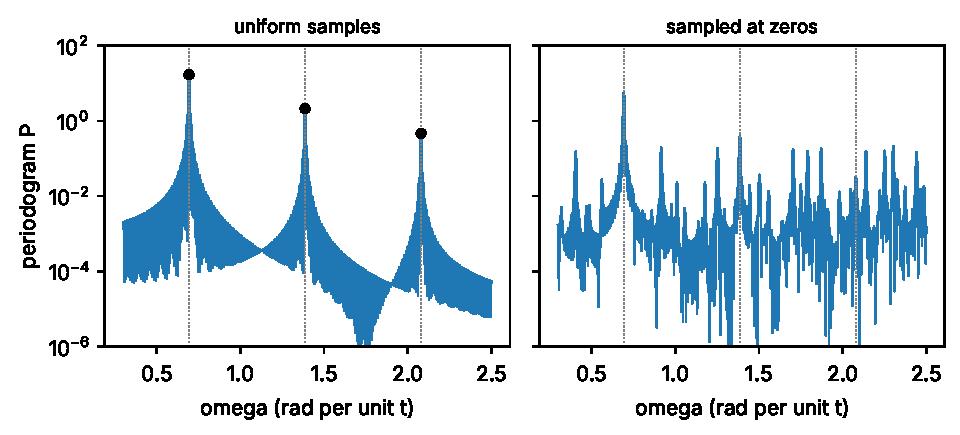
\includegraphics[width=0.95\linewidth]{figs/fourier-transform_re2.pdf}
\caption{Periodogram \eqref{eq:fourier-transform-periodogram} of the prime-2 wave RE2, $-\frac1\pi\sum_{m=1}^{3}\sin(mt\log2)/(m2^{m/2})$, on the range $t_1\le t\le t_{400}$ of zeros 1--400 (logarithmic vertical scale). Left: uniform samples at spacing $0.5$; dots mark the prediction $NA_m^2/4$. Right: the same function sampled only at the 400 zeros. Vertical lines: $m\log2$, $m=1,2,3$.}
\label{fig:fourier-transform-re2}
\end{figure}

\begin{pycode}
import numpy as np
import qmnt

t = qmnt.zeros(400)                       # t_1 ... t_400
n = np.arange(1, 401)
u = t/(2*np.pi)
y = n - 0.5 - (u*np.log(u) - u + 7/8)     # y_n = n - 1/2 - Nsm(t_n)
y = y - y.mean()                          # remove the omega = 0 line

def P(w):                                 # periodogram at one frequency
    return abs(np.sum(y*np.exp(-1j*w*t)))**2 / len(t)

T = t[-1] - t[0]                          # window length
step = 0.25*2*np.pi/T                     # a quarter of the resolution
w = np.arange(0.3, 3.0, step)             # coarse grid
Pw = np.array([P(v) for v in w])
k = np.argmax(Pw)                         # coarse peak
wf = np.linspace(w[k]-step, w[k]+step, 201)   # refine on 201 points
Pf = np.array([P(v) for v in wf])
w_peak = wf[np.argmax(Pf)]
print(w_peak, np.log(2), 2*np.pi/T)       # peak lies within 2*pi/T of log 2
\end{pycode}

\subsection{The periodogram of the zeros}

Now the real thing. Define, as in the paper's Sec.~II~D, the quantity
\begin{equation}
y_n=n-\tfrac12-N_{\rm sm}(t_n),
\label{eq:fourier-transform-yn}
\end{equation}
where $N_{\rm sm}$ is the smooth counting function of paper Eq.~(1) (Chapter~\ref{ch:counting-zeros}). The counting function $N(t)$ jumps from $n-1$ to $n$ at $t_n$; $n-\tfrac12$ is the midpoint of the jump, so $y_n$ is the fluctuating part $S=N-N_{\rm sm}$ read off at the $n$-th zero. Chapter~\ref{ch:explicit-formula} explains why $S$ is approximated by the prime sum $N_{\rm fl}$ of paper Eq.~(4). If that is right, the periodogram of $y_n$ sampled at the $t_n$ should show lines at $\log p^m$. \Cref{fig:fourier-transform-zerospec} shows it does. The tallest peak in $0.3<\omega<3$ sits at $\log2$, within the resolution $2\pi/T$ of this 1000-zero window. Within $2\pi/T$ of each of $\log3$, $\log5$ and $\log7$ there is a peak more than three times the median level of the periodogram over this range. The dashed lines mark further prime powers for comparison.

\begin{figure}[htbp]\centering
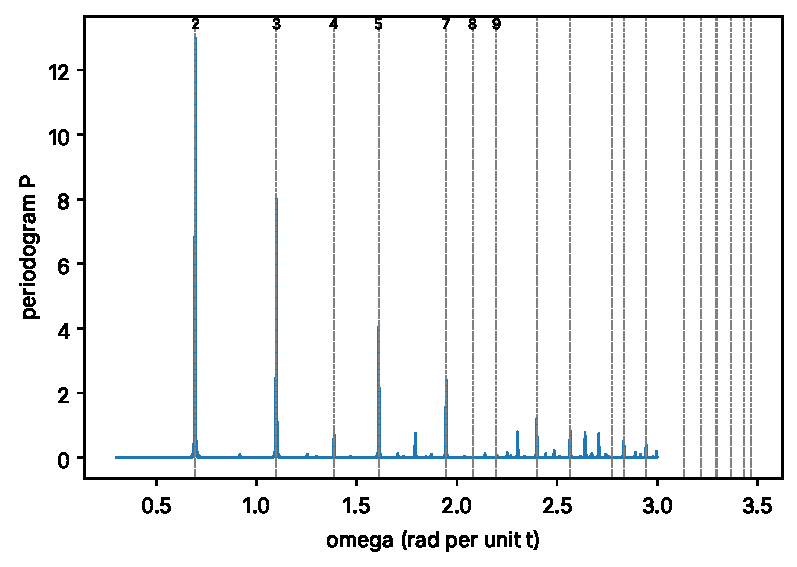
\includegraphics[width=0.85\linewidth]{figs/fourier-transform_zerospec.pdf}
\caption{Periodogram of the fluctuation $y_n=n-\frac12-N_{\rm sm}(t_n)$ of the first 1000 zeros, computed as the direct sum \eqref{eq:fourier-transform-periodogram} at the irregular points $t_n$ (mean subtracted). Dashed vertical lines mark $\log q$ for prime powers $q\le36$; the first few are labeled. The tallest peak is at $\log 2$.}
\label{fig:fourier-transform-zerospec}
\end{figure}

\begin{checkpoint}
The line heights $NA^2/4$ in \eqref{eq:fourier-transform-lineheight} grow with $N$, but the noise level \eqref{eq:fourier-transform-noise} does not. Does that mean that with enough data you can resolve $\log127$ from $\log128$ even though $T<801$?
\end{checkpoint}
\checkanswer{No. More samples in the same window raise the peaks above the noise, but resolution depends only on the window length $T$, Eq.~\eqref{eq:fourier-transform-resolution}. Two lines closer than about $2\pi/T$ merge into one peak no matter how many samples you take.}

\begin{keyideas}

\item The periodogram $P(\omega)=\abs{\sum y_je^{-i\omega t_j}}^2/N$, Eq.~\eqref{eq:fourier-transform-periodogram}, works for any sampling; subtract the mean first.
\item A line of amplitude $A$ reaches $\approx NA^2/4$; white noise sits at $\sigma^2$; the ratio $NA^2/(4\sigma^2)$ grows with $N$, Eq.~\eqref{eq:fourier-transform-snr}. The amplitude estimate is $2\abs F/N$.
\item Search on a coarse grid finer than one bin (a quarter bin loses at most $2.6\%$ of amplitude), then refine.
\item The periodogram of the zeros' fluctuation has its peaks at $\log p^m$, the tallest at $\log 2$.

\end{keyideas}

%======================================================================
\section{Power spectrum, autocorrelation and the Wiener--Khinchin theorem}\label{sec:fourier-transform-wk}
% DYK-BEGIN
\begin{didyouknow}{Einstein Got There First}
The Wiener-Khinchin theorem says that the power spectrum of a fluctuating signal is the Fourier transform of its autocorrelation. Norbert Wiener proved it in 1930 and Aleksandr Khinchin in 1934. Yet Albert Einstein had stated the essential idea in a short 1914 paper on analyzing irregularly fluctuating observations. His note went largely unnoticed for decades.
\end{didyouknow}
% DYK-END

The periodogram keeps the \emph{size} $\abs{X_k}$ of each Fourier coefficient and throws away its \emph{phase}. What, exactly, does it still know about the sequence? The answer is: its autocorrelation, and nothing else. The list of squared moduli $\abs{X_k}^2$ is called the \textbf{power spectrum} of the sequence; equivalently one can use the periodogram $P_k=\abs{X_k}^2/N$. The name ``power'' comes from Parseval's relation: these numbers, divided by $N$, add up to the sum of squares of the data.

\subsection{Autocorrelation}

The \textbf{autocorrelation} measures how much a sequence resembles a shifted copy of itself. For a real sequence $x_0,\dots,x_{N-1}$ and an integer lag $m$, define the \emph{ordinary} (lagged-product) autocorrelation
\begin{equation}
c_m=\sum_{j=0}^{N-1-m}x_j\,x_{j+m},\qquad m=0,1,\dots,N-1,
\label{eq:fourier-transform-acf}
\end{equation}
and the \emph{circular} autocorrelation, in which the sequence is wrapped around on itself,
\begin{equation}
r_m=\sum_{j=0}^{N-1}x_j\,x_{(j+m)\bmod N}.
\label{eq:fourier-transform-circacf}
\end{equation}
Here $a\bmod N$ is the remainder of $a$ on division by $N$. (The letters are reused: $c_m$ and $r_m$ here are not the Fourier coefficients $c_k$ of Section~\ref{sec:fourier-transform-def}, nor the ratio $r$ of a geometric series.) For lags $m$ small compared with $N$, the two differ only by the $m$ wrap-around terms. In data analysis one usually subtracts the mean first and divides by $c_0$, to get the normalized autocorrelation $c_m/c_0$, which equals 1 at lag 0. A positive value at lag $m$ means values $m$ steps apart tend to have the same sign; a negative value means they tend to have opposite signs. The fluctuations of the zeros have negative autocorrelation at lags 1--3, as the paper reports in Sec.~III; \cref{fig:fourier-transform-surrogate} shows this for zeros 1--400.

\subsection{The theorem}

\textbf{Wiener--Khinchin theorem (discrete, proved here).} For a real sequence $x$ with DFT $X$, the DFT of the circular autocorrelation is the squared modulus of the DFT:
\begin{equation}
R_k=\sum_{m=0}^{N-1}r_m\,e^{-2\pi imk/N}=\abs{X_k}^2 .
\label{eq:fourier-transform-wk}
\end{equation}
\emph{Proof.} Write $w=e^{-2\pi i/N}$. Substitute \eqref{eq:fourier-transform-circacf}:
\[R_k=\sum_{m=0}^{N-1}\sum_{l=0}^{N-1}x_l\,x_{(l+m)\bmod N}\,w^{mk}.\]
Fix $l$ and replace the summation variable $m$ by $j=(l+m)\bmod N$. As $m$ runs over $0,\dots,N-1$, so does $j$, each value once. Since $m$ and $j-l$ differ by a multiple of $N$ and $w^N=1$, we have $w^{mk}=w^{(j-l)k}=w^{jk}w^{-lk}$. Therefore
\[R_k=\sum_{l}\sum_{j}x_l\,x_j\,w^{jk}w^{-lk}=\Bigl(\sum_jx_jw^{jk}\Bigr)\Bigl(\sum_lx_lw^{-lk}\Bigr)=X_k\,\overline{X_k}=\abs{X_k}^2,\]
where the second factor is $\overline{X_k}$ because $x_l$ is real and $\overline{w}=w^{-1}$. $\square$

By the inverse DFT \eqref{eq:fourier-transform-idft}, $r_m=\frac1N\sum_k\abs{X_k}^2e^{2\pi imk/N}$: the autocorrelation is completely determined by the periodogram, and vice versa. Setting $m=0$ gives $r_0=\sum_jx_j^2=\frac1N\sum_k\abs{X_k}^2$, which is Parseval's relation \eqref{eq:fourier-transform-parseval} for real $x$. (For complex $x$, replace $x_lx_{l+m}$ by $\overline{x_l}x_{l+m}$; the same proof goes through.)

\textbf{Getting the ordinary autocorrelation.} Append $N$ zeros to $x$, making a sequence $\tilde x$ of length $2N$. For $0\le m<N$, a term $\tilde x_j\tilde x_{(j+m)\bmod 2N}$ of its circular autocorrelation is nonzero only if $j\le N-1$ and the second index is $\le N-1$. Since $j+m\le2N-2<2N$, no wrap-around occurs, so the second index is $j+m$, and we need $j\le N-1-m$. That leaves exactly the terms of $c_m$ in \eqref{eq:fourier-transform-acf}. So: zero-pad, FFT, take $\abs{\cdot}^2$, inverse FFT, keep lags $0,\dots,N-1$. This is how autocorrelations of long sequences are computed in practice.

\begin{sample}{Wiener--Khinchin by hand}
For $x=(1,1,0,0)$ compute the circular autocorrelation $r$, its DFT $R$, and $\abs{X_k}^2$, and confirm \eqref{eq:fourier-transform-wk}.

\textbf{Step 1: Autocorrelation.} Using \eqref{eq:fourier-transform-circacf} with $N=4$:
\begin{align*}
r_0&=1+1+0+0=2,\\
r_1&=x_0x_1+x_1x_2+x_2x_3+x_3x_0=1+0+0+0=1,\\
r_2&=x_0x_2+x_1x_3+x_2x_0+x_3x_1=0,\\
r_3&=x_0x_3+x_1x_0+x_2x_1+x_3x_2=0+1+0+0=1.
\end{align*}
So $r=(2,1,0,1)$. This is the sequence of the earlier DFT Sample Problem, so $R=(4,2,0,2)$.

\textbf{Step 2: DFT of $x$.} With phases $(-i)^{jk}$: $X_0=2$, $X_1=1+(-i)=1-i$, $X_2=1+(-1)=0$, $X_3=1+(-i)^3=1+i$.

\textbf{Step 3: Squared moduli.} $\abs{X_0}^2=4$, $\abs{1-i}^2=2$, $0$, $\abs{1+i}^2=2$: $(4,2,0,2)$. They agree.

\[\boxed{r=(2,1,0,1),\qquad R=\abs X^2=(4,2,0,2).}\]
\end{sample}

\begin{beyond}
\textbf{Taken on trust: the continuous Wiener--Khinchin theorem.} For a signal that fluctuates forever in a statistically steady way (a ``stationary random process''), the power spectral density is the Fourier transform of the autocorrelation function. The precise statement needs probability theory beyond this book; see the discussion of correlation functions and energy spectra in \cite{rhb}. Everything we use in this book is the discrete version \eqref{eq:fourier-transform-wk}, which we proved.
\end{beyond}

\textbf{What the power spectrum does not know.} The periodogram fixes the $\abs{X_k}$ but not the phases. Different phases give different sequences with the same periodogram and therefore, by \eqref{eq:fourier-transform-wk}, the same circular autocorrelation. The shift property is the simplest example: a circularly shifted sequence has $X_k$ multiplied by a phase factor and the same $\abs{X_k}$. But there are many more, as the next section exploits.

\begin{checkpoint}
Two real sequences of the same length have identical periodograms at every DFT frequency. Must they be identical? Must they have the same circular autocorrelation? The same sum of squares?
\end{checkpoint}
\checkanswer{They need not be identical (the phases may differ; a circular shift is one example). They must have the same circular autocorrelation, by Eq.~\eqref{eq:fourier-transform-wk} and the inverse DFT, and hence the same sum of squares $r_0$.}

\begin{keyideas}

\item The autocorrelation (ordinary \eqref{eq:fourier-transform-acf} or circular \eqref{eq:fourier-transform-circacf}) measures self-similarity under shifts; the zeros' fluctuations are negatively autocorrelated at lags 1--3.
\item Discrete Wiener--Khinchin, proved: the DFT of the circular autocorrelation is $\abs{X_k}^2$, Eq.~\eqref{eq:fourier-transform-wk}. Parseval is its $m=0$ case. Zero padding gives the ordinary autocorrelation.
\item The periodogram and the autocorrelation carry the same information; neither knows the phases.

\end{keyideas}

%======================================================================
\section{Phase randomization and surrogate data}\label{sec:fourier-transform-surrogates}

Suppose a model fits your data well. Is it using some specific structure in the data, or would it fit \emph{anything} with the same general look? One way to find out is to build fake data sets, \textbf{surrogates}, that share some properties with the real data and lack others, and then run the same analysis on them. If the model does just as well on the surrogates, it is not using what the surrogates lack. Theiler and collaborators \cite{theiler} introduced a now-standard surrogate: keep the amplitudes of the Fourier coefficients and scramble their phases.

\subsection{The recipe}

Start from a real sequence $x_0,\dots,x_{N-1}$ with DFT $X_k$.
\begin{enumerate}
\item For each $k$ with $1\le k<N/2$, choose an angle $\varphi_k$ uniformly at random in $[0,2\pi)$ and set $X'_k=X_ke^{i\varphi_k}$.
\item Keep $X'_0=X_0$, and, if $N$ is even, $X'_{N/2}=X_{N/2}$.
\item For $N/2<k\le N-1$, set $X'_k=\overline{X'_{N-k}}$, to restore the symmetry \eqref{eq:fourier-transform-dftsym}.
\item Invert: $x'_j=\frac1N\sum_kX'_ke^{2\pi ijk/N}$.
\end{enumerate}

\textbf{The result is real.} Conjugate step 4 and use step 3, $\overline{X'_k}=X'_{N-k}$ (which also holds for $k=0$ and $k=N/2$, because those are real and $N-0\equiv0$):
\[\overline{x'_j}=\frac1N\sum_k\overline{X'_k}e^{-2\pi ijk/N}=\frac1N\sum_kX'_{N-k}e^{-2\pi ijk/N}.\]
Let $k'=N-k$ (and $k'=0$ when $k=0$). Then $e^{-2\pi ijk/N}=e^{-2\pi ij(N-k')/N}=e^{2\pi ijk'/N}$, so the sum is $\frac1N\sum_{k'}X'_{k'}e^{2\pi ijk'/N}=x'_j$. A number equal to its own conjugate is real.

\textbf{What is preserved, exactly.}
\begin{itemize}
\item Every amplitude: $\abs{X'_k}=\abs{X_k}\abs{e^{i\varphi_k}}=\abs{X_k}$. Hence the periodogram, at every DFT frequency.
\item The circular autocorrelation, by the Wiener--Khinchin theorem \eqref{eq:fourier-transform-wk} and the uniqueness of the inverse DFT; and so, for lags small compared with $N$, approximately the ordinary one.
\item The mean, since $X'_0=X_0=\sum x_j$; and the sum of squares, which is $r_0$.
\end{itemize}

\textbf{What is destroyed.}
\begin{itemize}
\item All phase relations between frequency components, and with them any structure that is not captured by the power spectrum. If the data were, say, a sum of sinusoids all of whose phases are fixed by a law (the explicit formula has every term a pure sine, zero at $t=0$), that law is gone.
\item The \emph{distribution of values} (the ``marginal''). The surrogate's histogram generally differs from the original's, as the next Sample Problem shows. As a heuristic, a sum of many oscillations with random phases tends toward a bell-shaped (Gaussian) histogram (Chapter~\ref{ch:probability}).
\end{itemize}

\begin{sample}{Phase randomization by hand}
Phase-randomize $x=(1,1,0,0)$, choosing the random angle to be $\varphi_1=\pi/4$. As we will see, the new coefficient $X'_1$ then has phase $0$. Check that the result has the same circular autocorrelation but different values.

\textbf{Step 1: Coefficients.} From the previous Sample Problem, $X=(2,\,1-i,\,0,\,1+i)$. Only $X_1$ (and its mirror $X_3$) can be rotated; $X_0=2$ and $X_2=0$ stay. Since $X_1=1-i=\sqrt2\,e^{-i\pi/4}$, step 1 of the recipe gives $X'_1=X_1e^{i\varphi_1}=\sqrt2\,e^{-i\pi/4}e^{i\pi/4}=\sqrt2$, so $X'_3=\overline{X'_1}=\sqrt2$.

\textbf{Step 2: Invert.} With $N=4$, $e^{2\pi ijk/4}=e^{i\pi jk/2}$:
\[x'_j=\tfrac14\bigl[2+\sqrt2\,e^{i\pi j/2}+0+\sqrt2\,e^{3i\pi j/2}\bigr]=\tfrac14\bigl[2+\sqrt2\,(e^{i\pi j/2}+e^{-i\pi j/2})\bigr]=\tfrac12+\tfrac{\sqrt2}{2}\cos\frac{\pi j}{2},\]
using $e^{3i\pi j/2}=e^{-i\pi j/2}e^{2\pi ij}=e^{-i\pi j/2}$.

\textbf{Step 3: Values.} $\cos(\pi j/2)=1,0,-1,0$ for $j=0,1,2,3$, so $x'=(1.2071,\ 0.5,\ -0.2071,\ 0.5)$.

\textbf{Step 4: Check.} $r'_0=1.2071^2+0.25+0.0429+0.25=2.000$ and $r'_1=1.2071(0.5)+0.5(-0.2071)+(-0.2071)(0.5)+0.5(1.2071)=1.000$, equal to $r_0=2$, $r_1=1$. (By symmetry $r'_3=r'_1$, and $r'_2=0$; Problem~18 asks you to confirm.) But the original took only the values 0 and 1; the surrogate takes three different values ($1.2071$, $0.5$ twice, and $-0.2071$), one of them negative.

\[\boxed{x'=(1.2071,\,0.5,\,-0.2071,\,0.5):\ \text{same autocorrelation }(2,1,0,1),\ \text{different values}.}\]
\end{sample}

(Had we chosen $\varphi_1=\pi/2$ instead, so that $X'_1=\sqrt2\,e^{i\pi/4}$ has phase $\pi/4$, Step 2 would give $x'=(1,0,0,1)$: just a circular shift of $x$. A random phase gives, in general, something genuinely new.)

\begin{pycode}
import numpy as np

def phase_randomize(x, rng):
    """Real surrogate with the same |DFT| as x and random phases."""
    N = len(x)
    X = np.fft.rfft(x)                 # independent half: X_0 ... X_{N//2}
    phi = rng.uniform(0, 2*np.pi, len(X))
    phi[0] = 0.0                       # keep X_0 (the mean)
    if N % 2 == 0:
        phi[-1] = 0.0                  # keep the real coefficient X_{N/2}
    return np.fft.irfft(X*np.exp(1j*phi), n=N)   # irfft restores symmetry

def circ_autocorr(x):                  # Wiener--Khinchin in one line
    return np.fft.ifft(np.abs(np.fft.fft(x))**2).real

rng = np.random.default_rng(1)         # a seed makes the draw reproducible
x = np.array([1.0, 1.0, 0.0, 0.0])
xs = phase_randomize(x, rng)
print(xs)
print(circ_autocorr(x), circ_autocorr(xs))           # identical
print(np.abs(np.fft.fft(x)), np.abs(np.fft.fft(xs)))  # identical
\end{pycode}

\subsection{Two relatives}

\emph{Random permutation.} Shuffle the order of the values. This keeps the marginal distribution exactly (the same numbers, rearranged) and destroys the serial structure, including the autocorrelation. It is the opposite trade to phase randomization.

\emph{Amplitude-adjusted surrogates.} Schreiber and Schmitz \cite{schreiber} gave an iterative algorithm (IAAFT) that alternates between imposing the original Fourier amplitudes and imposing the original set of values, ending with a sequence that has exactly the original marginal and very nearly the original spectrum. Chapter~\ref{ch:controls} treats all three and the null hypotheses they test.

\begin{figure}[htbp]\centering
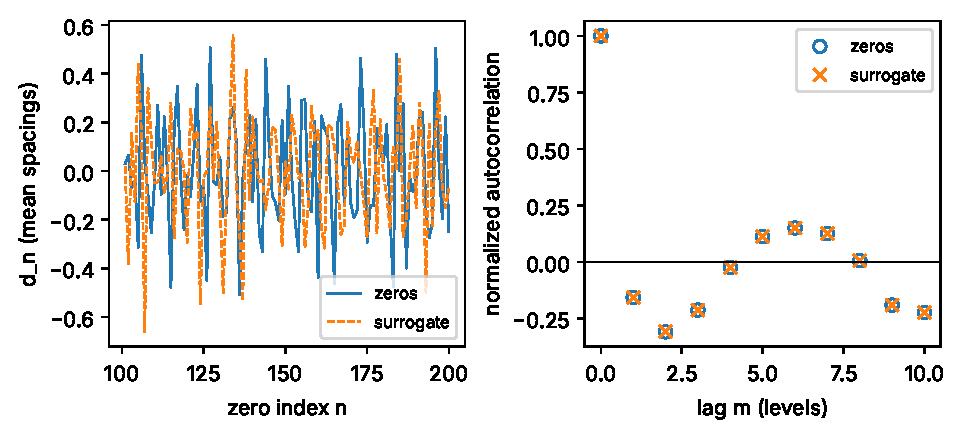
\includegraphics[width=0.95\linewidth]{figs/fourier-transform_surrogate.pdf}
\caption{Left: the fluctuation $d_n=(t_n-s_n)/\mathrm{gap}_n$ of zeros 101--200 in mean spacings (solid) and the same stretch of one phase-randomized surrogate of the full sequence $n\le400$ (dashed, seed 1). Right: normalized circular autocorrelation of the mean-subtracted sequences of length 400, real (circles) and surrogate (crosses); they coincide exactly, including the negative values at lags 1--3.}
\label{fig:fourier-transform-surrogate}
\end{figure}

\begin{checkpoint}
Which surrogate keeps the histogram of the data exactly, random permutation or phase randomization? Which keeps the autocorrelation exactly?
\end{checkpoint}
\checkanswer{Random permutation keeps the histogram (the same values in a new order) but destroys the autocorrelation. Phase randomization keeps the circular autocorrelation and periodogram exactly but changes the histogram.}

\begin{keyideas}

\item Phase randomization multiplies each $X_k$ ($0<k<N/2$) by a random $e^{i\varphi_k}$, restores the conjugate symmetry and inverts; the result is real.
\item It preserves the periodogram, the circular autocorrelation, the mean and the sum of squares exactly, and destroys phase structure and the marginal distribution.
\item Random permutation makes the opposite trade; IAAFT \cite{schreiber} keeps the marginal exactly and the spectrum nearly. Surrogates tell you which properties of the data a method actually uses.

\end{keyideas}

%======================================================================
\section{The spectrum of the zeros: a first look at Landau's formula}\label{sec:fourier-transform-landau}

So far we have Fourier-analyzed a \emph{function} ($y_n$) sampled at the zeros. A different and very striking object is the spectral window of the zeros themselves,
\begin{equation}
W(\omega)=\sum_{n:\,t_n\le T}e^{i\omega t_n},
\label{eq:fourier-transform-zerowin}
\end{equation}
the Fourier transform of the set of zeros up to height $T$. (Careful: here, following the usual statement of Landau's formula, $T$ is the \emph{height} of the top of the range, not the window length. The paper uses $T$ for the training window, for the tensors $T^{(n)}$ and for the Chebyshev polynomials $T_k$. Since $t_1=14.13$, the height and the window length differ by about 14, which is negligible for large $T$. The sign in the exponent is reversed from \eqref{eq:fourier-transform-specwin}; by (P2) this only conjugates the result.)

If the zeros were scattered at random, \eqref{eq:fourier-transform-zerowin} would be a featureless floor away from $\omega=0$. It is not.

\subsection{A heuristic derivation}

Let $N(t)$ be the number of zeros with $0<t_n\le t$ (Chapter~\ref{ch:counting-zeros}). Careful: in this section $N(t)$ is the zero-counting function, not the number of samples. Later, $x$ denotes a number greater than 1 (a prime power at the resonances), not a data sequence. Pick a height $t_a$ below $t_1$, so $N(t_a)=0$, and let $g(t)$ be any smooth function.

\emph{Step A (exact): summation by parts.} For each zero $t_n\le T$, $\int_{t_a}^{T}g'(t)\,[t\ge t_n]\,\dd t=g(T)-g(t_n)$, where $[t\ge t_n]$ is 1 for $t\ge t_n$ and 0 otherwise. Since $N(t)=\sum_n[t\ge t_n]$, summing over the $N(T)$ zeros gives $\int_{t_a}^Tg'N\,\dd t=N(T)g(T)-\sum_ng(t_n)$, so
\begin{equation}
\sum_{n:\,t_n\le T}g(t_n)=g(T)N(T)-\int_{t_a}^{T}g'(t)\,N(t)\,\dd t .
\label{eq:fourier-transform-sbp}
\end{equation}

\emph{Step B (exact): split $N$.} Write $N=N_{\rm sm}+S$, with $N_{\rm sm}$ of paper Eq.~(1) and $S$ the fluctuating part. Integrating the $N_{\rm sm}$ piece by parts once more, $\int g'N_{\rm sm}=[gN_{\rm sm}]_{t_a}^T-\int gN_{\rm sm}'$, so
\begin{equation}
\sum_{t_n\le T}g(t_n)=g(T)S(T)+g(t_a)N_{\rm sm}(t_a)+\int_{t_a}^{T}g\,N'_{\rm sm}\,\dd t-\int_{t_a}^{T}g'\,S\,\dd t .
\end{equation}
The derivative of Eq.~(1) is
\[N'_{\rm sm}(t)=\frac{1}{2\pi}\log\frac{t}{2\pi}+\frac{t}{2\pi}\cdot\frac1t-\frac1{2\pi}=\frac{1}{2\pi}\log\frac{t}{2\pi},\]
the average number of zeros per unit height (this is the density quoted in Section~\ref{sec:fourier-transform-sampling}).

\emph{Step C: take $g(t)=e^{i\omega t}$ with $\omega>0$.} The second term, $g(t_a)N_{\rm sm}(t_a)$, is a constant that does not depend on $T$. The first term has modulus $\abs{S(T)}$. Numerically $\abs S$ is typically below 1 at these heights (Chapter~\ref{ch:counting-zeros}). In general it can grow, but only slowly: $S(T)=\order(\log T)$ is a proved bound whose proof is beyond this book (see \cite{titchmarsh}). Either way this term is small compared with $T$.

For the integral of $e^{i\omega t}N'_{\rm sm}$, integrate by parts once more, using $\frac{\dd}{\dd t}\frac{e^{i\omega t}}{i\omega}=e^{i\omega t}$ and
\[N''_{\rm sm}(t)=\frac{\dd}{\dd t}\Bigl(\frac{1}{2\pi}\log\frac{t}{2\pi}\Bigr)=\frac{1}{2\pi t}:\]
\[\int_{t_a}^{T}e^{i\omega t}N'_{\rm sm}\,\dd t=\Bigl[\frac{e^{i\omega t}}{i\omega}N'_{\rm sm}(t)\Bigr]_{t_a}^{T}-\frac{1}{i\omega}\int_{t_a}^{T}\frac{e^{i\omega t}}{2\pi t}\,\dd t .\]
The boundary terms have moduli $\frac{1}{2\pi\omega}\abs{\log\frac{T}{2\pi}}$ and $\frac{1}{2\pi\omega}\abs{\log\frac{t_a}{2\pi}}$, using $\abs{e^{i\omega t}}=1$. The last integral has modulus at most $\frac{1}{2\pi\omega}\int_{t_a}^{T}\frac{\dd t}{t}=\frac{1}{2\pi\omega}\log\frac{T}{t_a}$, by the bound $\abs{\int g}\le\int\abs g$ of Section~\ref{sec:fourier-transform-def}. So the whole integral is of order $\frac{1}{\omega}\log T$, tiny compared with $T$. The interesting term is $-\int g'S\,\dd t=-i\omega\int e^{i\omega t}S(t)\,\dd t$.

\emph{Step D (heuristic): replace $S$ by the explicit formula.} Anticipating Chapter~\ref{ch:explicit-formula}, take $S(t)\approx-\frac1\pi\sum_{p}\sum_{m}\frac{\sin(mt\log p)}{mp^{m/2}}$ (paper Eq.~(4) with all primes). Suppose $\omega=\log x$ with $x=p^m$ a prime power. The matching (``resonant'') term contributes
\[-i\omega\cdot\left(-\frac{1}{\pi mp^{m/2}}\right)\int_{t_a}^{T}e^{i\omega t}\sin(\omega t)\,\dd t .\]
Since $e^{i\omega t}\sin\omega t=\cos\omega t\sin\omega t+i\sin^2\omega t$ and $\sin^2=\frac12(1-\cos2\omega t)$, the integral is $iT/2$ plus bounded oscillating pieces (we neglect the small $t_a$). So the resonant contribution is
\[\frac{i\omega}{\pi mp^{m/2}}\cdot\frac{iT}{2}=-\frac{\omega T}{2\pi mp^{m/2}}=-\frac{T}{2\pi}\cdot\frac{m\log p}{mp^{m/2}}=-\frac{T}{2\pi}\,\frac{\log p}{\sqrt x},\]
using $\omega=\log x=m\log p$ and $p^{m/2}=\sqrt x$. Each non-resonant term gives a bounded contribution that does not grow with $T$. With the \textbf{von Mangoldt function} $\Lambda(x)=\log p$ if $x=p^m$ is a prime power and $\Lambda(x)=0$ otherwise (Chapter~\ref{ch:primes}),
\begin{equation}
\sum_{t_n\le T}e^{i t_n\log x}\approx-\frac{T}{2\pi}\,\frac{\Lambda(x)}{\sqrt x}\qquad(x>1).
\label{eq:fourier-transform-landau}
\end{equation}
Step D is heuristic: the prime sum does not converge on the critical line, and the infinitely many non-resonant terms are not controlled. Nevertheless a precise version of the conclusion is a theorem (box below). It is stated as a sum of $x^\rho$ over the zeros $\rho$. It turns into \eqref{eq:fourier-transform-landau}, with an additional error of order $\log T$ (divided by $\sqrt x$), at every height up to which all zeros are known to lie on the critical line. This has been verified numerically for all the zeros used in this book. This error grows far more slowly than the main term, which is proportional to $T$.

\begin{beyond}
\textbf{Taken on trust: Landau's formula.} For fixed $x>1$,
\[\sum_{0<\Im\rho\le T}x^{\rho}=-\frac{T}{2\pi}\Lambda(x)+\order(\log T),\]
where the sum runs over all nontrivial zeros $\rho$ of zeta with imaginary part in $(0,T]$. In this form it is a theorem, and it does \emph{not} assume that the zeros lie on the critical line. Now suppose every zero up to height $T$ has the form $\rho_n=\frac12+it_n$. This is verified numerically for all zeros used in this book; that it holds at every height is the Riemann hypothesis, which is open. Then $x^{\rho_n}=x^{1/2}e^{it_n\log x}$ (Chapter~\ref{ch:complex}), and dividing by $\sqrt x$ gives \eqref{eq:fourier-transform-landau} plus an error $\order(\log T)/\sqrt x$. The proof is in Landau's 1912 paper \cite{landau}; Gonek \cite{gonek} gave a version uniform in $x$.
\end{beyond}

So the zeros' spectrum has spikes, growing linearly in $T$, exactly at $\omega=\log p^m$, and nowhere else (apart from $\omega=0$). Notice the weight: the periodogram of the \emph{fluctuation} $y_n$ has lines of size $\propto1/(mp^{m/2})$, decreasing with $p$, while the zeros' own spectrum has spikes $\propto\log p/p^{m/2}$. The extra factor $\omega=m\log p$ came from $g'$ in Step C: counting zeros is like differentiating the counting function.

\begin{sample}{How tall is the $\log 2$ spike for the first 1000 zeros?}
Use \eqref{eq:fourier-transform-landau} with $T=t_{1000}=1419.42$ (paper Sec.~II~A) to predict $\sum_{n\le1000}\cos(t_n\log x)$ for $x=2$ and $x=3$, and compare with the value $1000$ at $\omega=0$.

\textbf{Step 1: Prefactor.} $T/2\pi=1419.42/6.2832=225.91$.

\textbf{Step 2: $x=2$.} $\Lambda(2)/\sqrt2=0.69315/1.41421=0.49013$, so the prediction is $-225.91\times0.49013=-110.7$.

\textbf{Step 3: $x=3$.} $\Lambda(3)/\sqrt3=1.09861/1.73205=0.63428$, prediction $-143.3$.

\textbf{Step 4: Compare.} At $\omega=0$ every term is 1, so the sum is $1000$. The $\log 2$ spike is about $11\%$ of that, which is far above what random points would give (of order $\sqrt{1000}\approx32$). A direct computation with \texttt{qmnt} (the listing below, and \cref{fig:fourier-transform-landau}) gives $-111.1$ at $\log2$, within $1\%$ of the prediction. Agreement this close is partly fortunate, and should not be expected in general. Landau's theorem (box above) has an error term of order $\log T$ with an unspecified constant, and $\log t_{1000}=7.26$, while the main term is only about $111$. Problem~25 repeats the comparison at the much larger height $t_{10000}$.

\[\boxed{\textstyle\sum_{n\le1000}\cos(t_n\log2)\approx-110.7,\qquad\sum_{n\le1000}\cos(t_n\log3)\approx-143.3.}\]
\end{sample}

\begin{figure}[htbp]\centering
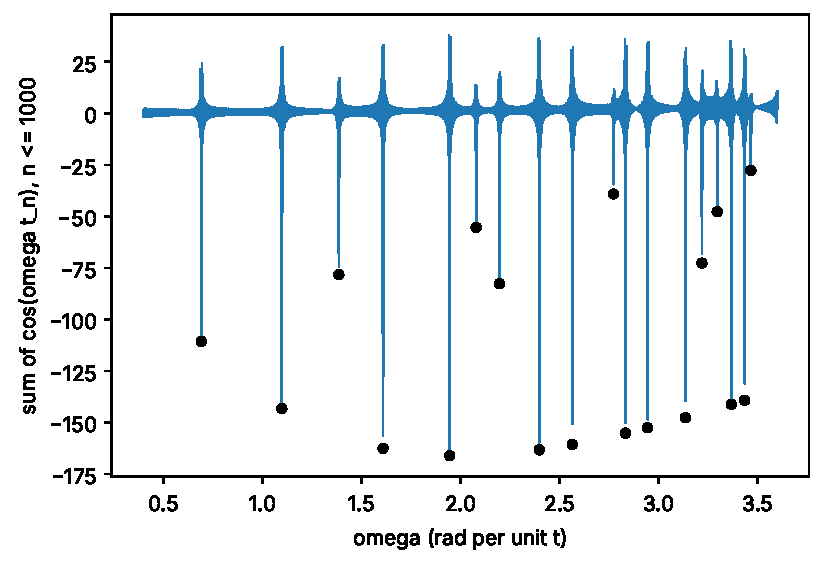
\includegraphics[width=0.85\linewidth]{figs/fourier-transform_landau.pdf}
\caption{The real part of the spectral window of the zeros, $\sum_{n\le1000}\cos(\omega t_n)$, for $0.4\le\omega\le3.6$. Downward spikes appear at $\omega=\log q$ for prime powers $q$; dots mark Landau's prediction $-(T/2\pi)\Lambda(q)/\sqrt q$ of Eq.~\eqref{eq:fourier-transform-landau} with $T=t_{1000}$. At $\omega=0$ (off the plot) the sum is 1000.}
\label{fig:fourier-transform-landau}
\end{figure}

\begin{pycode}
import numpy as np
import qmnt

t = qmnt.zeros(1000)
T = t[-1]                                   # height of the top zero
for x, Lam in [(2, np.log(2)), (3, np.log(3)), (4, np.log(2)), (5, np.log(5))]:
    w = np.log(x)
    measured = np.sum(np.cos(w*t))
    predicted = -(T/(2*np.pi))*Lam/np.sqrt(x)
    print(x, round(measured, 1), round(predicted, 1))
\end{pycode}

Two consequences for this chapter's tools. First, when you sample a function at the zeros, the spectral window $W$ of \eqref{eq:fourier-transform-specwin} has these spikes, so a line at $\omega_0$ reappears weakly at $\omega_0\pm\log q$; for $T=t_{1000}$ the strongest such echoes (at $\log5$, $\log7$, $\log11$, where $\Lambda(q)/\sqrt q$ is largest) are about a sixth of the main line. Second, it is the reason the fluctuation of the zeros is \emph{predictable} by an arithmetic formula, the theme of Chapters~\ref{ch:explicit-formula} and~\ref{ch:paper-arithmetic}.

\begin{checkpoint}
Is the spectral window of the zeros flat away from $\omega=0$, as it would roughly be for random points?
\end{checkpoint}
\checkanswer{No. By Landau's formula it has spikes of depth about $(T/2\pi)\Lambda(q)/\sqrt q$ at every $\omega=\log q$ with $q$ a prime power, growing linearly with the height $T$.}

\begin{keyideas}

\item Summation by parts, Eq.~\eqref{eq:fourier-transform-sbp}, turns sums over zeros into integrals against $N=N_{\rm sm}+S$; the average density of zeros is $\frac1{2\pi}\log\frac t{2\pi}$.
\item Landau's formula (a theorem; proof beyond this book): for fixed $x>1$, $\sum_{0<\Im\rho\le T}x^{\rho}=-\frac{T}{2\pi}\Lambda(x)+\order(\log T)$. Where all zeros up to height $T$ lie on the critical line (verified numerically for the zeros used here), dividing by $\sqrt x$ gives Eq.~\eqref{eq:fourier-transform-landau} plus an error $\order(\log T)/\sqrt x$. The zeros' spectrum is concentrated at $\log p^m$.
\item Our derivation of it from the explicit formula is heuristic; the size $\propto\log p/p^{m/2}$ differs from the $1/(mp^{m/2})$ of the fluctuation's lines by the factor $\omega$.

\end{keyideas}

%======================================================================
\section{Paper connection}\label{sec:fourier-transform-paper}

Here is where each tool of this chapter enters the paper \cite{soniR1}. Section and equation numbers refer to revision R1.

\subsection{The fitted sinusoidal controls of Sec.~II~D}

Sec.~II~D (paragraph ``Fitted sinusoidal controls'') introduces models of the form $N_{\rm sm}(t)+F(t)=n-\frac12$ with $F(t)=\sum_j[a_j\sin(\omega_jt)+b_j\cos(\omega_jt)]$, trained by least squares on exactly the quantity $y_n=n-\frac12-N_{\rm sm}(t_n)$ of our Eq.~\eqref{eq:fourier-transform-yn}, at the training zeros only. The fitting is linear least squares, the subject of Chapter~\ref{ch:least-squares}; the choice of frequencies is Fourier analysis.

\textbf{C1: a uniform frequency grid.} ``450 frequencies on a uniform grid (900 coefficients)'', with $\omega_j=8j/450$ (App.~A step 20). The grid spacing is $8/450=0.01778$. For the fit on zeros 1--400 the Fourier resolution is $2\pi/T\approx0.0094$ (Sample Problem ``Resolving prime-power frequencies''), so the grid spacing is about $1.9$ resolution elements. The grid treats every frequency from $0$ to $8$ alike; it has no preference for $\log p^m$. A line at $\log q$ generally falls between grid points, and by \eqref{eq:fourier-transform-indist} the nearest grid frequency, up to $0.0089$ away, drifts out of phase with it by up to $0.0089\times666\approx6$ radians across the window, so the model must build each line from several grid components. Table~IV reports C1 at $0.258$ with correlation $+0.28$ on zeros 401--500 (Sec.~IV gives the correlation interval $[+0.08,+0.46]$), against a null of $0.263$: ``capacity without a suitable prior does not generalize'' (Sec.~IV). Why this happens is a question about extrapolating fitted combinations outside the window, which Chapter~\ref{ch:sparse-frequency} analyzes.

\textbf{C2: a periodogram peak search.} ``A sparse model whose $K$ frequencies are found one at a time as the largest peak of the periodogram of the current residual on $0.05<\omega<8$, with all amplitudes refitted after each addition ($3K$ parameters)'' (Sec.~II~D). Every ingredient is in Section~\ref{sec:fourier-transform-periodogram}: the periodogram \eqref{eq:fourier-transform-periodogram} computed by a direct sum at the irregular points $t_n$; a search range; a coarse grid with ``step a quarter of $2\pi/T$'' and ``refinement on 201 points'' (App.~A step 20). Our Sample Problem showed that a quarter-bin step catches at least $97.4\%$ of any isolated line's amplitude. For the 400-zero window the coarse grid over $0.05<\omega<8$ has a little under 3400 points. The three parameters per frequency are $\omega_j$, $a_j$ and $b_j$. The procedure of subtracting the fit and searching the residual's periodogram again is a form of matching pursuit, developed in Chapter~\ref{ch:sparse-frequency}; ridge strength and $K$ are chosen by a forward split inside the training window, also treated there. The paper reports that C2 ``selects 24 frequencies (72 parameters) from 400 zeros and predicts zeros 401--500 at $0.034$ with correlation $+0.99$'', and from 800 zeros selects 43 frequencies and scores $0.034/{+0.99}$ on 801--1000 (Sec.~IV, Table~IV). \Cref{fig:fourier-transform-zerospec} shows why such a search can work: the periodogram of $y_n$ is dominated by peaks at $\log p^m$.

\textbf{Frequencies above the ``equivalent Nyquist''.} For the 800-zero fit, the paper lists the matched prime powers: ``those up to 113 except 32, 64, and 81, and six primes between 131 and 211'' (Sec.~IV). Now $\log211=5.35$, while the equivalent Nyquist frequency of the zeros at the top of that window is $\pi/\mathrm{gap}=\frac12\log(s_{800}/2\pi)\approx2.62$ (Section~\ref{sec:fourier-transform-sampling}). Uniformly spaced samples could not have distinguished these frequencies from aliases below $2.62$. That the search recovered them is a numerical observation of the paper. It is compatible with the fact (Section~\ref{sec:fourier-transform-sampling}) that irregular sampling breaks exact aliasing. However, the zeros are not random sample points, and the mechanism is not established here. We claim nothing beyond this compatibility.

\subsection{``Within half the Fourier resolution'' and the alignment check}

Sec.~IV states: ``Every selected frequency lies within half the Fourier resolution of the training window of the logarithm of a prime power.'' Half the Fourier resolution is $\pi/T$; App.~A step 23 makes this the matching criterion $\abs{\omega-\log q}<\pi/T$, with $q\le3000$. The upper limit fits the search range: $e^8=2981$, so $q\le3000$ covers every $\log q$ below the top of the range $\omega<8$. The criterion is exploratory by the paper's own account: the cutoff-maximized binomial score ($24.7$ and $50.9$ on the real zeros, at most $4.7$ on 900 surrogate replicates) was ``defined after the data were seen'' (App.~A step 23), and Sec.~IV states that ``no significance claim is made here beyond the size of the ensembles.'' One of the three surrogate families in step 23 is ``sorted phase-randomized surrogates''. The other two are sparse signals with non-arithmetic frequencies: explicit formulas with 25 displaced prime frequencies, and explicit-formula shapes with 25 random base frequencies. The phase randomization is the construction of Section~\ref{sec:fourier-transform-surrogates}. The sorting presumably restores an increasing list that can again be read as heights, but the paper does not spell this out. Why matching within $\pi/T$ is a sensible tolerance follows from Section~\ref{sec:fourier-transform-window}: for an isolated line the periodogram maximum lies at the line itself. Noise and the sidelobes of neighboring lines displace it by a fraction of the main-lobe half-width $2\pi/T$, so half a resolution element, $\pi/T$, is a reasonable tolerance. For the 400-zero window $\pi/T\approx0.0047$. Chapter~\ref{ch:sparse-frequency} discusses how often a random frequency would match some $\log q$ by chance, which is why surrogate replicates were needed at all.

\subsection{Shuffled and phase-randomized targets in Sec.~III}

The paragraph ``Permutation and surrogate tests'' of Sec.~III refits the operator protocol (scale 1, $M=400$, zeros 1--400) to targets in which the fluctuation sequence in mean spacings, $d_n=(\tilde t_n-E_n[\mathrm{smooth}])/\mathrm{gap}_n$ (App.~A step 18), is replaced by a random permutation (``marginal distribution kept, serial structure destroyed''), a phase-randomized surrogate \cite{theiler} (``power spectrum kept exactly, no arithmetic content'') or an IAAFT surrogate \cite{schreiber} (``marginal kept exactly, spectrum to 1\%''). These three phrases are precisely the preserved/destroyed lists of Section~\ref{sec:fourier-transform-surrogates}. Step 18 records the construction: ``real FFT, uniform phases'', seeds 1--10, which is our recipe with \texttt{rfft}/\texttt{irfft}. Note that the FFT is legitimate here because $d_n$ is indexed by the integer $n$ and is therefore uniformly sampled in $n$ (pitfall in Section~\ref{sec:fourier-transform-dft}).

The results: in-sample rms $0.134\pm0.010$, $0.141\pm0.006$ and $0.138\pm0.005$ over ten draws each, against $0.137$ for the true zeros and $0.244$ for the null (Sec.~III). The phase-randomized surrogates keep the autocorrelation of the true $d_n$, including the negative values at lags 1--3 that \cref{fig:fourier-transform-surrogate} shows, but destroy the arithmetic phase structure; the permuted ones destroy even the autocorrelation. The fit does equally well on all of them. In the paper's words, ``in-sample accuracy measures capacity, not captured structure.'' Phase randomization keeps the power spectrum of $d_n$, in frequency per level, because the FFT is taken over the index $n$. It scrambles the phases, however. So the specific arithmetic pattern in $t$, sines at $\log p^m$ with phases fixed by the explicit formula, is no longer present; the paper summarizes this as ``no arithmetic content''. Note that a line at frequency $\omega$ in $t$ is not a sharp line in $n$. Near level $n$ it advances by about $\omega\,\mathrm{gap}_n$ radians per level, and $\mathrm{gap}_n$ shrinks across the window, so its frequency per level drifts.

\subsection{Landau, Gonek and the line spectrum}

Sec.~IV writes: ``That the Fourier transform of the zeros is concentrated at logarithms of prime powers is classical \cite{landau,gonek}; C2 is a control built on that fact, not a new result.'' Section~\ref{sec:fourier-transform-landau} stated Landau's formula and checked it numerically (\cref{fig:fourier-transform-landau}). Keep the paper's hedge: C2 succeeds because ``sparse in $t$-frequency'' is ``itself a strong and well-chosen prior'' (Sec.~IV), and the facts of this chapter tell you why the prior is well chosen.

\subsection{Resolution and the decay of skill}

The paper notes that C2's ``skill also decays with distance from the training window as the estimated frequencies dephase ($0.078/{+0.96}$ on zeros 1001--2000 for the 400-zero fit), which the exact frequencies of the oracle do not'' (Sec.~IV). Inequality \eqref{eq:fourier-transform-indist} is the seed of this: a window of length $T$ fixes a frequency only to a fraction of $2\pi/T$, and an error $\delta\omega$ grows into a phase error $\delta\omega\,\Delta t$ at distance $\Delta t$. Chapter~\ref{ch:sparse-frequency} derives the consequences. The oracle of paper Eq.~(4) uses the exact $m\log p$ and has no such error, which is consistent with its nearly height-independent skill in Table~V.

\subsection{The continuation probe}

The ``Arithmetic-continuation probe'' of Sec.~III trains the operator on the prime-2 wave RE2 alone, a signal whose spectrum is three lines (Section~\ref{sec:fourier-transform-window}): it represents the window in-sample (rms $0.056$, correlation $+0.95$) and ``continues it not at all'' (held-out correlation $+0.07$). From the Fourier point of view, a model that knew ``three lines at $m\log2$'' would continue it exactly; Chapter~\ref{ch:fourier-series} showed why no finite window's periodic extension can. Figure~1 of the paper shows the same contrast on real data.

%======================================================================
\section{Summary}
% DYK-BEGIN
\begin{didyouknow}{Gauss Did the FFT}
The fast Fourier transform, published by James Cooley and John Tukey in 1965, cut the cost of a discrete Fourier transform of $N$ points from about $N^2$ to about $N\log N$ operations. Historians later found that Carl Friedrich Gauss had used essentially the same trick around 1805 to interpolate asteroid orbits. His Latin notes appeared only in his posthumous collected works.
\end{didyouknow}
% DYK-END

\begin{itemize}
\item Fourier transform $\hat f(\omega)=\int f e^{-i\omega t}\dd t$, Eq.~\eqref{eq:fourier-transform-def}, inverse Eq.~\eqref{eq:fourier-transform-inv} (proof beyond); properties P1--P5: linearity, $\hat f(-\omega)=\overline{\hat f(\omega)}$ for real $f$ \eqref{eq:fourier-transform-hermitian}, shift \eqref{eq:fourier-transform-shift}, modulation \eqref{eq:fourier-transform-modulation}, scaling.
\item A line seen through a window of length $T$ becomes $T\,\mathrm{sinc}((\omega-\omega_0)T/2)$, Eq.~\eqref{eq:fourier-transform-sinc}; resolution $2\pi/T$, Eq.~\eqref{eq:fourier-transform-resolution}; largest sidelobe $0.217$; Hann window \eqref{eq:fourier-transform-hann} has sidelobes $0.027$ but a doubled main lobe.
\item Almost periodic sums have line spectra, Eq.~\eqref{eq:fourier-transform-lines}; paper Eq.~(4) has lines at $\log p^m$ of size $1/(2\pi m p^{m/2})$.
\item Uniform sampling aliases $\omega$ with $\omega+2\pi/\Delta t$; Nyquist frequency $\pi/\Delta t$, Eq.~\eqref{eq:fourier-transform-nyquist}. Irregular samples: direct sum \eqref{eq:fourier-transform-directsum}, spectral window \eqref{eq:fourier-transform-specwin}.
\item DFT \eqref{eq:fourier-transform-dft}, inverse \eqref{eq:fourier-transform-idft} from orthogonality \eqref{eq:fourier-transform-orth}, symmetry \eqref{eq:fourier-transform-dftsym}, Parseval \eqref{eq:fourier-transform-parseval}; FFT cost $N\log_2N$.
\item Periodogram \eqref{eq:fourier-transform-periodogram}: line height $NA^2/4$, noise level $\sigma^2$, Eq.~\eqref{eq:fourier-transform-snr}; search on a sub-bin grid and refine.
\item Discrete Wiener--Khinchin, Eq.~\eqref{eq:fourier-transform-wk}: periodogram and circular autocorrelation carry the same information.
\item Phase randomization keeps $\abs{X_k}$, autocorrelation, mean and sum of squares; destroys phases and the marginal.
\item Landau's formula \eqref{eq:fourier-transform-landau}: the zeros' spectrum has spikes at $\log p^m$ of depth $\frac{T}{2\pi}\Lambda(x)/\sqrt x$.
\end{itemize}

%======================================================================
\section{Problems}

\begin{problemlist}
\prob{1}{Using the box transform of the first Sample Problem, find $\hat f(\omega)$ at $\omega=\pi/T$, as a multiple of $T$.}
\prob{1}{Samples are taken every $\Delta t=0.25$. Find the Nyquist frequency, and the frequency in $[0,\omega_{\rm N}]$ at which a component with $\omega=15$ appears.}
\prob{1}{What window length $T$ is needed to resolve $\log 3$ from $\log 4$ by the criterion \eqref{eq:fourier-transform-resolution}?}
\prob{1}{Compute the DFT of $x=(1,0,0,0)$ and check Parseval's relation.}
\prob{1}{For $N=2^{20}$, find the speed-up factor of the FFT over the direct DFT.}
\prob{2}{For $f=e^{-a\abs t}$ with $a=2$, find $\hat f(0)$ and the FWHM. Verify that the product (FWHM)$\times(1/a)$ is the same as for $a=0.5$.}
\prob{2}{Show that observing $e^{i\omega_0 t}$ on $[0,T]$ instead of $[-T/2,T/2]$ gives a transform with the same modulus as Eq.~\eqref{eq:fourier-transform-sinc}, and find the extra phase factor.}
\prob{2}{A sinusoid of amplitude $A=0.05$ is buried in white noise of rms $\sigma=0.5$, with $N=1000$ samples. Estimate the ratio of its periodogram peak to the mean noise level.}
\prob{2}{Compute the DFT of $x=(1,-1,1,-1)$. Which frequency is present, and why is it the Nyquist frequency?}
\prob{2}{Show that the Hann expression \eqref{eq:fourier-transform-hann} tends to $\frac14$ as $\delta\to1$. (Use $\sin(\pi\delta)\approx-\pi(\delta-1)$ near $\delta=1$.)}
\prob{2}{A coarse grid has step one half of a bin. Find the worst-case fraction of a line's amplitude seen on the grid (rectangular window).}
\prob{2}{(Paper.) For the 400-zero window, compare $\abs{\log128-\log127}$ with the matching tolerance $\pi/T$ of App.~A step 23 and with the resolution $2\pi/T$. What does this say about whether the search could distinguish these two prime powers?}
\prob{2}{(Paper.) For the fit on zeros 1--800, take $T=t_{800}-t_1$. Using \texttt{qmnt}, find $2\pi/T$ and the ratio of the C1 grid spacing $8/450$ to it.}
\prob{2}{(Computational.) Using \texttt{qmnt} and \texttt{numpy}, compute the periodogram of RE2 sampled at zeros 1--400 and list the three largest local maxima in $0.3<\omega<2.5$. Compare their positions with $m\log2$.}
\prob{2}{Use Landau's formula \eqref{eq:fourier-transform-landau} with $T=t_{1000}$ to predict $\sum_{n\le1000}\cos(t_n\log 4)$.}
\prob{2}{Explain why the mean should be subtracted before computing a periodogram, using the size $N\bar y^2$ of the line at $\omega=0$ and the sidelobes of the spectral window.}
\prob{2}{(Computational.) Using \texttt{numpy}, phase-randomize $d_n=$\texttt{qmnt.fluct}$(t_n,n)$ for $n\le400$ with seeds 1--10. Verify that the circular autocorrelation is unchanged and compare the largest value of $\abs{d_n}$ before and after.}
\prob{2}{Complete the phase-randomization Sample Problem: verify that $r'_2=0$ and $r'_3=1$ for $x'=(1.2071,0.5,-0.2071,0.5)$.}
\prob{2}{(Paper.) Sec.~III reports in-sample rms $0.134$, $0.141$, $0.138$ on permuted, phase-randomized and IAAFT targets, $0.137$ on the true zeros and $0.244$ for the null. Compute the fraction of the null removed in each case, and say what this does and does not show.}
\prob{2}{For $x=(1,1,0,0)$ compute the ordinary autocorrelation $c_m$ of \eqref{eq:fourier-transform-acf} and compare with the circular $r_m$. Then verify the zero-padding recipe by computing the circular autocorrelation of $(1,1,0,0,0,0,0,0)$ at lags $0$--$3$.}
\prob{3}{Prove Parseval's relation \eqref{eq:fourier-transform-parseval} directly from the orthogonality relation \eqref{eq:fourier-transform-orth}, for complex $x$.}
\prob{3}{Show from \eqref{eq:fourier-transform-hann} that the Hann sidelobes fall like $1/\abs\delta^3$ for large $\abs\delta$ and find the constant.}
\prob{3}{(Paper.) Compute the equivalent Nyquist frequency $\frac12\log(s_{1000}/2\pi)$ at the top of the 1000-zero range used for the operator fits, and compare with $\log 211$.}
\prob{3}{Show that if $t_j=j\Delta t$, the samples of $e^{i\omega t}$ and $e^{i(\omega+2\pi k/\Delta t)t}$ coincide for every integer $k$, and that for real cosines $\cos(\omega t)$ and $\cos((2\pi/\Delta t-\omega)t)$ coincide.}
\prob{3}{(Computational.) Using \texttt{qmnt.zeros(10000)}, compute $\sum_{n\le10^4}\cos(t_n\log2)$ and compare with Landau's prediction for $T=t_{10000}$.}
\end{problemlist}

%======================================================================
\section{Answers to selected problems}

\textbf{1.} $\hat f(\pi/T)=2\sin(\pi/2)/(\pi/T)=2T/\pi\approx0.637\,T$.

\textbf{2.} $\omega_{\rm N}=\pi/0.25=12.57$. The alias period is $2\pi/0.25=25.13$; $15$ is confused with $25.13-15=10.13$.

\textbf{3.} $\log(4/3)=0.2877$, so $T\gtrsim2\pi/0.2877=21.8$.

\textbf{4.} Every phase factor multiplies $x_0=1$ only at $j=0$, so $X_k=1$ for all $k$: $X=(1,1,1,1)$. Parseval: $1=\frac14(4)$.

\textbf{5.} $N^2/(N\log_2N)=N/\log_2N=2^{20}/20=52428.8$, a speed-up of about $5\times10^4$.

\textbf{7.} Let $g_c$ be the centered windowed oscillation of Eq.~\eqref{eq:fourier-transform-sinc}, and let $g$ be the one observed on $[0,T]$.

For $0\le t\le T$ we have $g_c(t-T/2)=e^{i\omega_0(t-T/2)}$. Hence $g(t)=e^{i\omega_0T/2}\,g_c(t-T/2)$ for every $t$, since both sides vanish outside $[0,T]$.

By linearity (P1) and the shift property \eqref{eq:fourier-transform-shift} with $t_0=T/2$,
\[\hat g(\omega)=e^{i\omega_0T/2}e^{-i\omega T/2}\hat g_c(\omega)=e^{-i(\omega-\omega_0)T/2}\,\hat g_c(\omega).\]
The extra phase factor $e^{-i(\omega-\omega_0)T/2}$ has modulus 1, so $\abs{\hat g}=\abs{\hat g_c}$.

\textbf{9.} $x_j=(-1)^j=e^{i\pi j}$, so only $k=2$ survives: $X=(0,0,4,0)$. The frequency $\omega_2=2\cdot2\pi/(4\Delta t)=\pi/\Delta t$, two samples per cycle, is the Nyquist frequency.

\textbf{11.} With a step of half a bin, the worst offset is a quarter bin. Then $s(\frac14)=\sin(\pi/4)/(\pi/4)=0.9003$, that is, $90.0\%$ of the amplitude.

\textbf{13.} With \texttt{qmnt}, $T=t_{800}-t_1\approx1169$, so $2\pi/T\approx0.0054$; the C1 grid spacing $0.01778$ is about $3.3$ resolution elements. A generic grid becomes coarser relative to the resolution as the window grows.

\textbf{15.} $\Lambda(4)=\log2$, $\sqrt4=2$: prediction $-225.91\times0.34657=-78.3$.

\textbf{17.} The circular autocorrelations agree to rounding error for all seeds (Wiener--Khinchin). The largest $\abs{d_n}$ changes from draw to draw: the marginal distribution is not preserved, which is why IAAFT \cite{schreiber} exists.

\textbf{19.} Fractions of the null removed: $1-0.134/0.244=45\%$, $42\%$, $43\%$, against $44\%$ for the true zeros. The fit gains the same on targets that lack the arithmetic phase structure (and, for permutation, the autocorrelation). It shows the in-sample gain measures capacity; it does not by itself show anything about held-out skill, which Sec.~III tests separately.

\textbf{20.} $c=(2,1,0,0)$ while $r=(2,1,0,1)$: $c_3=x_0x_3=0$, whereas $r_3$ also contains the wrap-around terms $x_1x_0+x_2x_1+x_3x_2$, of which $x_1x_0=1$. Padded: $(2,1,0,0)$ at lags $0$--$3$, equal to $c$.

\textbf{21.} $\sum_k\abs{X_k}^2=\sum_k\sum_j\sum_l x_j\overline{x_l}e^{-2\pi ik(j-l)/N}=\sum_j\sum_lx_j\overline{x_l}\,N[j=l]=N\sum_j\abs{x_j}^2$, using \eqref{eq:fourier-transform-orth} with $m=l-j$.

\textbf{23.} $s_{1000}\approx1419.4$, so $\frac12\log(s_{1000}/2\pi)\approx2.71$, below $\log211=5.35$ by a factor of about 2.

\textbf{25.} With $t_{10000}\approx9.88\times10^3$ from \texttt{qmnt.zeros(10000)}, Landau's prediction is $-(t_{10000}/2\pi)\log2/\sqrt2\approx-770.5$. The listing of Section~\ref{sec:fourier-transform-landau}, with 1000 replaced by 10000, gives a measured sum of about $-771.6$. The relative discrepancy $\abs{\text{measured}-\text{predicted}}/\abs{\text{predicted}}$ is $0.14\%$, against $0.35\%$ at $T=t_{1000}$. The theorem's error term is $\order(\log T)$ while the main term grows like $T$, so the relative error \emph{bound} shrinks with height. A single height is not guaranteed to show a smaller discrepancy, because the constant in the error term is not specified.
